% !TeX spellcheck = en_US
%%%%%%%%%%%%%%%%%%%%%%%%%%%%%%%%%%%%%%%%%
% Masters/Doctoral Thesis 
% LaTeX Template
% Version 2.2 (21/11/15)
%
% This template has been downloaded from:
% http://www.LaTeXTemplates.com
%
% Version 2.x major modifications by:
% Vel (vel@latextemplates.com)
%
% This template is based on a template by:
% Steve Gunn (http://users.ecs.soton.ac.uk/srg/softwaretools/document/templates/)
% Sunil Patel (http://www.sunilpatel.co.uk/thesis-template/)
%
% Template license:
% CC BY-NC-SA 3.0 (http://creativecommons.org/licenses/by-nc-sa/3.0/)
%
%%%%%%%%%%%%%%%%%%%%%%%%%%%%%%%%%%%%%%%%%

%----------------------------------------------------------------------------------------
%	PACKAGES AND OTHER DOCUMENT CONFIGURATIONS
%----------------------------------------------------------------------------------------

\documentclass[
12pt, % The default document font size, options: 10pt, 11pt, 12pt
oneside, % Two side (alternating margins) for binding by default, uncomment to switch to one side
english, % ngerman for German
onehalfspacing, % Single line spacing, alternatives: onehalfspacing or doublespacing
%draft, % Uncomment to enable draft mode (no pictures, no links, overfull hboxes indicated)
%nolistspacing, % If the document is onehalfspacing or doublespacing, uncomment this to set spacing in lists to single
%liststotoc, % Uncomment to add the list of figures/tables/etc to the table of contents
%toctotoc, % Uncomment to add the main table of contents to the table of contents
%parskip, % Uncomment to add space between paragraphs
%nohyperref, % Uncomment to not load the hyperref package
headsepline, % Uncomment to get a line under the header
]{MastersDoctoralThesis} % The class file specifying the document structure

\usepackage{pdfx}
\usepackage[utf8]{inputenc} % Required for inputting international characters
%\usepackage[T1]{fontenc} % Output font encoding for international characters

%\usepackage{palatino} % Use the Palatino font by default

\usepackage[backend=bibtex,style=numeric,natbib=true,sorting=none,maxbibnames=199,minbibnames=10,maxcitenames=10,firstinits=true]{biblatex} % User the bibtex backend with the authoryear citation style (which resembles APA)
%\usepackage{biblatex}

\addbibresource{refs.bib} % The filename of the bibliography

\usepackage[autostyle=true]{csquotes} % Required to generate language-dependent quotes in the bibliography


\usepackage{graphicx}
\usepackage{subfigure}


\usepackage{float}  
 

\usepackage{amsmath}
\usepackage{cleveref}
\usepackage{amssymb}
\usepackage{amsfonts}
\usepackage{siunitx}
\usepackage{tabularx} 
\usepackage{bbm}
\usepackage{epstopdf}
%\usepackage[]{bibentry}

%\usepackage{showframe}
\graphicspath{ {images/} }
\newcommand{\virgolette}[1]{``#1''}
\newcommand{\minus}{\scalebox{0.35}[0.65]{$-$}}
%\renewcommand{\floatpagefraction}{.7}
%\renewcommand{\topfraction}{0.3}
%\renewcommand{\textfraction }{0.05}
%\renewcommand{\topfraction}{0.9}

%\renewcommand\floatpagefraction{.8}
%\renewcommand\dblfloatpagefraction{.8} % for two column documents
%\renewcommand\topfraction{.8}
%\renewcommand\dbltopfraction{.8} % for two column documents
%\renewcommand\bottomfraction{.8}
%\renewcommand\textfraction{.05}

%%\includeonly{./TeX_files/predicting}
%\includeonly{frontespizio}

%----------------------------------------------------------------------------------------
%	MARGIN SETTINGS
%----------------------------------------------------------------------------------------

\geometry{
	paper=a4paper, % Change to letterpaper for US letter
	%inner=2.5cm, % Inner margin
	%outer=3.8cm, % Outer margin
	%bindingoffset=2cm, % Binding offset
	inner=3cm, % Inner margin
	outer=3cm, % Outer margin
	top=3cm, % Top margin
	bottom=3cm, % Bottom margin
	%showframe,% show how the type block is set on the page
}

%----------------------------------------------------------------------------------------
%	THESIS INFORMATION
%----------------------------------------------------------------------------------------

\thesistitle{Methods for Sentiment Analysis and Social Media Popularity\\of Crowdsourced Visual Contents} % Your thesis title, this is used in the title and abstract, print it elsewhere with \ttitle
\supervisor{Sebastiano Battiato} % Your supervisor's name, this is used in the title page, print it elsewhere with \supname
%\examiner{} % Your examiner's name, this is not currently used anywhere in the template, print it elsewhere with \examname
\degree{Dottorato di Ricerca} % Your degree name, this is used in the title page and abstract, print it elsewhere with \degreename
\author{Alessandro Ortis} % Your name, this is used in the title page and abstract, print it elsewhere with \authorname
\addresses{} % Your address, this is not currently used anywhere in the template, print it elsewhere with \addressname

\subject{Subject Area} % Your subject area, this is not currently used anywhere in the template, print it elsewhere with \subjectname
\keywords{} % Keywords for your thesis, this is not currently used anywhere in the template, print it elsewhere with \keywordnames
\university{Università degli Studi di Catania} % Your university's name and URL, this is used in the title page and abstract, print it elsewhere with \univname
\department{Dipartimento di Matematica e InformaticaAAA} % Your department's name and URL, this is used in the title page and abstract, print it elsewhere with \deptname
\group{Image Processing Laboratory} % Your research group's name and URL, this is used in the title page, print it elsewhere with \groupname
%\faculty{\href{http://faculty.university.com}{Faculty Name}} % Your faculty's name and URL, this is used in the title page and abstract, print it elsewhere with \facname

\hypersetup{pdftitle=\ttitle} % Set the PDF's title to your title
\hypersetup{pdfauthor=\authorname} % Set the PDF's author to your name
\hypersetup{pdfkeywords=\keywordnames} % Set the PDF's keywords to your keywords

\newcommand{\ci}{\mathrel{\text{\scalebox{1.07}{$\perp\mkern-10mu\perp$}}}}

\begin{document}

\frontmatter % Use roman page numbering style (i, ii, iii, iv...) for the pre-content pages

\pagestyle{plain} % Default to the plain heading style until the thesis style is called for the body content

%----------------------------------------------------------------------------------------
%	TITLE PAGE
%----------------------------------------------------------------------------------------

%\begin{titlepage}
%\begin{center}
%
%\textsc{\LARGE \univname}\\[1.5cm] % University name
%\textsc{\Large Tesi di Dottorato di Ricerca}\\[0.5cm] % Thesis type
%
%\HRule \\[0.4cm] % Horizontal line
%{\huge \bfseries \ttitle}\\[0.4cm] % Thesis title
%\HRule \\[1.5cm] % Horizontal line
% 
%\begin{minipage}{0.4\textwidth}
%\begin{flushleft} \large
%\emph{Author:}\\
%\authorname
%%\href{http://www.johnsmith.com}{\authorname} % Author name - remove the \href bracket to remove the link
%\end{flushleft}
%\end{minipage}
%\begin{minipage}{0.4\textwidth}
%\begin{flushright} \large
%\emph{Supervisor:} \\
%\supname
%%\href{http://www.jamessmith.com}{\supname} % Supervisor name - remove the \href bracket to remove the link  
%\end{flushright}
%\end{minipage}\\[3cm]
% 
%\large \textit{A thesis submitted in fulfillment of the requirements\\ for the degree of \degreename}\\[0.3cm] % University requirement text
%\textit{in the}\\[0.4cm]
%\groupname\\\deptname\\[2cm] % Research group name and department name
% 
%{\large \today}\\[4cm] % Date
%%\includegraphics{Logo} % University/department logo - uncomment to place it
% 
%\vfill
%\end{center}
%\end{titlepage}

\begin{titlepage}
\centering 
%\includegraphics[height=2.565cm]{Figures/university_logo.png}
%\vspace*{2.565cm}

\bigskip

{\Large \textbf{UNIVERSIT\`A DEGLI STUDI DI CATANIA}}

{\scshape
\large
Dipartimento di Matematica e Informatica
}

{\scshape
\normalsize
Dottorato di Ricerca in Matematica e Informatica XXXI Ciclo
}

\bigskip


\hrule

\vspace{3cm}
\vspace{0.5cm}

{\itshape
\large
\authorname
\par}

\vspace{3.2cm}
%\vspace{0.5cm}

{\centering
\Large
\ttitle
\par}

\vspace{3cm}
%\vspace{0.5cm}


\begin{minipage}[b]{8 cm}
\hrule

\bigskip

{\centering\scshape 
Tesi di Dottorato di Ricerca
\par}


\bigskip

\hrule
\end{minipage}
%\bigskip


\bigskip



\bigskip


\bigskip


\bigskip


\bigskip


\bigskip

\vspace{1.5cm}

{\raggedleft
\begin{tabular}{ll}
\supname
\end{tabular}

\par}


\bigskip

\bigskip



\hrule

\bigskip

\vspace{0.5cm}

{\centering
Anno Accademico 2017 - 2018
\par}
\end{titlepage}


%----------------------------------------------------------------------------------------
%	DECLARATION PAGE
%----------------------------------------------------------------------------------------
%
%\begin{declaration}
%\addchaptertocentry{\authorshipname}
%
%\noindent I, \authorname, declare that this thesis titled, \enquote{\ttitle} and the work presented in it are my own. I confirm that:
%
%\begin{itemize} 
%\item This work was done wholly or mainly while in candidature for a research degree at this University.
%\item Where any part of this thesis has previously been submitted for a degree or any other qualification at this University or any other institution, this has been clearly stated.
%\item Where I have consulted the published work of others, this is always clearly attributed.
%\item Where I have quoted from the work of others, the source is always given. With the exception of such quotations, this thesis is entirely my own work.
%\item I have acknowledged all main sources of help.
%\item Where the thesis is based on work done by myself jointly with others, I have made clear exactly what was done by others and what I have contributed myself.\\
%\end{itemize}
% 
%\noindent Signed:\\
%\rule[0.5em]{25em}{0.5pt} % This prints a line for the signature
% 
%\noindent Date:\\
%\rule[0.5em]{25em}{0.5pt} % This prints a line to write the date
%\end{declaration}
%
%\cleardoublepage

%----------------------------------------------------------------------------------------
%	QUOTATION PAGE
%----------------------------------------------------------------------------------------

\vspace*{0.2\textheight}

\noindent\enquote{\itshape Quote.}\bigbreak

\hfill 

%----------------------------------------------------------------------------------------
%	ABSTRACT PAGE
%----------------------------------------------------------------------------------------

\begin{abstract}
\addchaptertocentry{\abstractname} % Add the abstract to the table of contents
Abstract.
\end{abstract}

%----------------------------------------------------------------------------------------
%	ACKNOWLEDGEMENTS
%----------------------------------------------------------------------------------------

\begin{acknowledgements}
\addchaptertocentry{\acknowledgementname} % Add the acknowledgements to the table of contents
Acknowledgements go here.
\end{acknowledgements}

%----------------------------------------------------------------------------------------
%	LIST OF CONTENTS/FIGURES/TABLES PAGES
%----------------------------------------------------------------------------------------

\tableofcontents % Prints the main table of contents

%\listoffigures % Prints the list of figures

%\listoftables % Prints the list of tables

%----------------------------------------------------------------------------------------
%	ABBREVIATIONS
%----------------------------------------------------------------------------------------
%
%\begin{abbreviations}{ll} % Include a list of abbreviations (a table of two columns)
%
%\textbf{LAH} & \textbf{L}ist \textbf{A}bbreviations \textbf{H}ere\\
%\textbf{WSF} & \textbf{W}hat (it) \textbf{S}tands \textbf{F}or\\
%
%\end{abbreviations}

%----------------------------------------------------------------------------------------
%	PHYSICAL CONSTANTS/OTHER DEFINITIONS
%----------------------------------------------------------------------------------------
%
%\begin{constants}{lr@{${}={}$}l} % The list of physical constants is a three column table
%
%% The \SI{}{} command is provided by the siunitx package, see its documentation for instructions on how to use it
%
%	Speed of Light & $c_{0}$ & \SI{2.99792458e8}{\meter\per\second} (exact)\\
%%Constant Name & $Symbol$ & $Constant Value$ with units\\
%
%\end{constants}

%----------------------------------------------------------------------------------------
%	SYMBOLS
%----------------------------------------------------------------------------------------
%
%\begin{symbols}{lll} % Include a list of Symbols (a three column table)
%
%$a$ & distance & \si{\meter} \\
%$P$ & power & \si{\watt} (\si{\joule\per\second}) \\
%%Symbol & Name & Unit \\
%
%\addlinespace % Gap to separate the Roman symbols from the Greek
%
%$\omega$ & angular frequency & \si{\radian} \\
%
%\end{symbols}

%----------------------------------------------------------------------------------------
%	DEDICATION
%----------------------------------------------------------------------------------------
%
%\dedicatory{Dedicated to myself, and whatever I will be} 

%----------------------------------------------------------------------------------------
%	THESIS CONTENT - CHAPTERS
%----------------------------------------------------------------------------------------

\mainmatter % Begin numeric (1,2,3...) page numbering

\pagestyle{thesis} % Return the page headers back to the "thesis" style

% Include the chapters of the thesis as separate files from the Chapters folder
% Uncomment the lines as you write the chapters

\chapter{Introduction}
- INTRODUZIONE DELLA TESI E DEL LAVORO DI DOTTORATO (VEDI FIL)
- INTRODUZIONE SOMMARIA DEI PROBLEMI AFFRONTATI (CHE VERRA' POI APPROFONDITA IN CIASCUNA SECTION)

%% FILTRARE LA SEGUENTE INTRODUZIONE (CSUR18) 
Nowadays, the amount of public available information encourages the study and development of algorithms that analyse huge amount of users' data with the aim to infer reactions about topics, opinions, trends and to understand the mood of the users whose produce and share information through the web. The aim of Sentiment Analysis is to extract the attitude of people toward a topic or the intended emotional affect the author wishes to have on the readers. The tasks of this research field are challenging as well as very useful in practice. Sentiment analysis finds several practical applications, since opinions influence many human decisions either in business and social activities.  
\\
ALLARGARE LE CATEGORIE DI TASK, INSERENDO LE DIVERSE ACCEZIONI DI SENTIMENT 
\\
SENTIMENT  ---> CONTENT POLARITY AND CONTENT POPULARITY
\\POLARITY   ---> POSITIVE / NEGATIVE EVOKED EMOTION ---> SENTIMENT PREDICTION
\\POPULARITY ---> POPULARITY ON SOCIAL PLATFORMS --> FLICKR
\\POPULARITY ---> POPULARITY IN SOCIAL EVENTS --> RECFUSION + TSP

Sentiment analysis systems are being applied in almost every business and social domain because opinions are central to almost all human activities and are key influencers of our behaviours. 

Although NLP (Natural Language Processing) offers several approaches to address the problem of understanding users' preferences and behaviours, the social media context offers some additional challenges. Beside the huge amounts of available data, typically the textual communications on social networks consist of short and colloquial messages. Moreover, people tend to use also images and videos, in addition to the textual messages, to express their experiences through the most common social platforms.
The information contained in such visual contents are not only related to semantic information such as objects or actions about the acquired picture, but also cues about affect and sentiment conveyed by the depicted scene. Such information is hence useful to understand the emotional impact (i.e., the evoked sentiment) beyond the semantic.
For these reasons images and videos have become one of the most popular media by which people express their emotions and share their experiences in the social networks, which have assumed a crucial role in collecting data about people's opinions and feelings. 
Images and videos produced by users and shared in social media platforms reflect visual aspects of users' daily activities and interests. Such growing user generated images represent a recent and powerful source of information useful to analyse users' interests. 
%Extracting the emotions inherently underlying images perceived by the viewers could promote new approaches to several application fields such as brand perception, assessment of customer satisfaction, advertising, and media analytic, etc.
%The diffusion of personal mobile devices constantly connected to Internet services (e.g., smartphones) and the growth of social media platforms introduced a new communication paradigm by which people that share multimedia data. %, by allowing new interaction models. 
In this context, uploading images and videos to a social media platform is the new way by which people share their opinions and experiences.  
This provides a strong motivation for research on this field, and offers many challenging research problems.

This dissertation we present several scientific works that analyses images and videos produced by users in a social context (i.e., a social platform, a social event or a public site), with the aim to infer user's interests and behaviours.


\section{Dissertation Structure}
\begin{figure}[t]
	\centering
	%	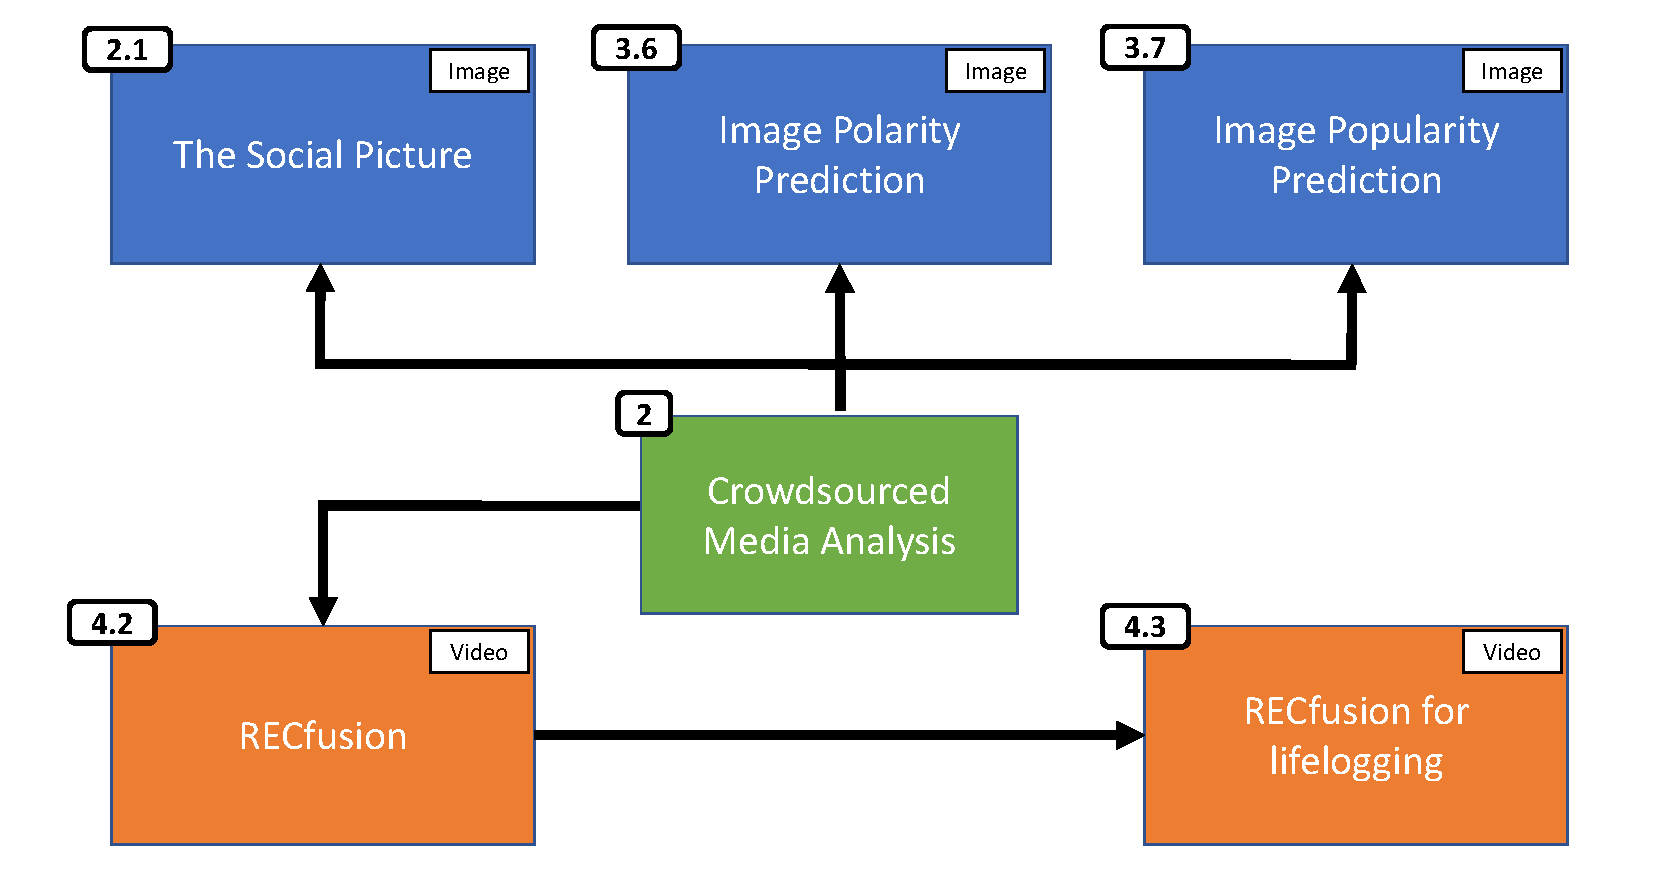
\includegraphics[width=1\linewidth]{schema.pdf}
	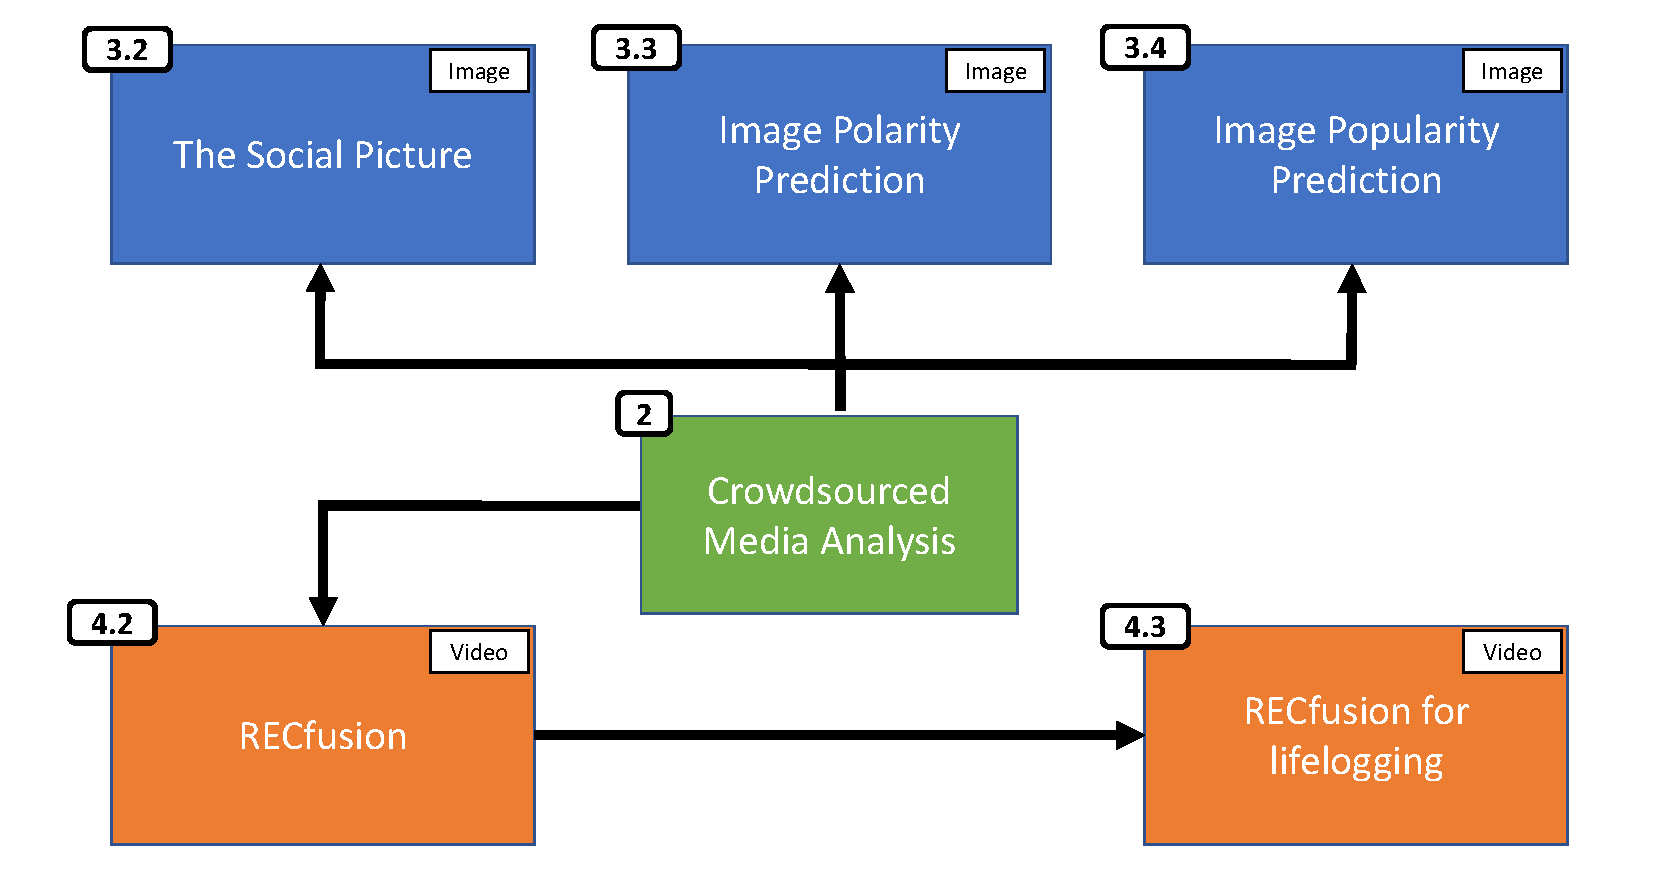
\includegraphics[width=0.8\linewidth]{schema2.pdf}
	\caption{Dissertation structure. Numbers depicts the Sections which describe the proposed work. Blue blocks represent algorithms that work on images, whereas orange blocks represent algorithms that work on videos. All the media involved in the works presented in this dissertation are produced by users.
	}
	\label{figDissertationSchema}
\end{figure}
In this dissertation, titled \virgolette{Methods for Sentiment Analysis and Social Media Popularity of Crowdsourced Visual Contents}, we mainly treated image and video contents produced by groups of users (i.e., crowded).
For this reason, the dissertation is properly divided into three main parts: Crowdsourced Media Analysis, Image Sentiment Analysis and Video Sentiment Analysis.
The dissertation structure is shown in Figure~\ref{figDissertationSchema}. We start our discussion by an introduction on Crowdsourced Media Analysis, which brings together all the works presented in this dissertation. Each algorithm is presented in a different Section. In Chapter~\ref{ch3}, we present all the methods that analyses images for the tasks of users behaviour analysis, image polarity prediction and image popularity prediction.
In Chapter~\ref{ch4}, we present our works related to the analysis of video contents.
In this research work, the sentiment associated to images has been studied under several meanings. Hence, different research questions have been addressed. 
One is to understand the most popular subjects related to a place or an event, by the analysis of the images produced by users visiting that place or attending the event. This study produced two main framework: \textit{The Social Picture} and \textit{RECfusion}. The first framework is aimed to understand user preferences based on the pictures taken from users themselves in the context of a specific event or place. The output of \textit{The Social Picture} is a set of statistical insights about the collected images, as well as some exploration tools which allow to understand the most important subjects. The second is aimed to understand what is the scene recorded simultaneously by the most number of users attending the same event, based on the videos taken from the users at the same time. The output of \textit{RECfusion} is a video depicting the most popular scene over time composed by segments of videos selected from the users' ones.
The approach defined in \textit{RECfusion} has been further improved and extended to the First Person View (PFV) video domain, for the task of daily monitoring for assistive lifelogging.



\section{List of Publications}
\chapter{Crowdsourced Media Analysis}\label{ch2}
With the rapid growth in communication technology, both companies and research institutes have been given the opportunity to perform large scale analysis on a multitude of real user-generated data, with a huge variety of application contexts.
Crowdsourcing provides the opportunity for input from a number of sources, with different degrees of granularity, and allows to find new ways to reach audiences on a broader scale. %Moreover, the growing industry of online communication through smartphones provides a way for people of all backgrounds to give input on a project or research.
%Sometimes the possibility to participate on a project, or just express their opinions encourages people to partecipate to crowdsourcing campains.
%Often times, the trigger to attract a huge amount of contributors is the so called ``gamification''.
Social media, blogs, forums, comment sections in online websites allow the opportunity for people to give suggestions or concerns.

There are three main assets that supported the rise of the ``crowdsourcing era'':
\begin{itemize}
	\item \textbf{Social Platforms}: the diffusion of social networks plays a crucial role in collecting information about people opinion, trends and behaviour. There are general social networks like Facebook where people chat, read news, and share their experiences. Furthermore, there are also very specific social platforms aimed to bring together people with common interests. There are platforms by which computer engineers share code and advices, or professional photographers can share their photos, etc. What happens now is that people love sharing their information, tell friends what they are doing and how they feel. And what is very important for the scientific community is that most of these information are public and immediately available.
	\item \textbf{High Bandwidth Connection}: the number of people with an Internet connection is increasing, as well as the bandwidth and the available connection speed. With the 5G connection, it's possible to download an high quality two hour long movie in less than 4 seconds. 
	The connectivity improvements allowed the development of new services based on the transmission of huge amount of data, and real-time services. This allowed, for instance, web-based services like Netflix and the IP television, with the possibility to watch movies or live events with very high quality and low latency, or to perform a video of the event the user is attending, allowing him to share the live streaming through a social network.
	\item \textbf{Personal Devices}: the diffusion of personal devices like smartphones allows people to be connected in every second of their lives, wherever they are in that moment. This allows the users to access on-line services in any moment of their daytime. Moreover, the amount of personal data that can be acquired by personal devices allow these services to be more pervasive and user centric.% Moreover, with the huge amount of available personal data, the provided services became more pervasive and user specific (i.e., more persuasive, and attractive). 
\end{itemize}

%Companies have caught on to the attention surrounding crowdsourcing, and have sought out innovative 
Companies have been attempting innovative ways to get their customers involved both in production and promotion processes of their products and services. Crowdsourcing brings people together through a web-based platform, %this allows brands access to untapped talent that might not be located in their area. Crowdsourcing 
generally by means of social media, so businesses can obtain insights about what topics consumers are talking about or are interested in.
%From asking followers their preference on a design or color scheme, all the way to submitting their own content, companies large and small have realized the benefits of using their most valuable asset (their customers) to test new ideas. 
Asking what people like before offering a new product on the market helps reduce the risk of a product or service failure, while also generating hype around a new offering.

In the last decade, several companies exploited the crowdsourcing paradigm to offer innovative services. For example, crowdsourcing has changed the way people travel. The rise of services like AirBnB, Uber, and what has been termed the ``sharing economy'', transformed what had been primarily a mass-produced experience into a peer-to-peer economic network.

Companies like AirBnB and Uber have driven down prices by increasing the marketplace offer. Customers also benefit from increased variety and personalization in their travel options. 
%Whereas in the past a traveller relied on known hotel and taxi brands to provide reliable experiences, nowadays they are just as likely to tap into the marketplace that one of those new companies facilitates (Uber, AirBnB), and enjoy a more unique experience. 
The traveller’s issues and habits has remained rather the same, what have changed are only the service providers, and often times the service provided. %Rather than the traditional taxi to the airport, flight to a destination and taxi to the hotel pattern, a traveler these days is more likely to take an Uber (or Lyft) to the airport, fly to their destination, hop into another crowd-sourced vehicle, and head to the apartment they booked on AirBnB.
%Additionally, whereas in the past someone new to a city might rely on their hotel’s receptionist for restaurant recommendations, these days they are just as likely to ask Yelp, or even their AirBnB hosts.
Although the low prices can be attractive, the most of users trust the deals of such kind of companies due to the feedbacks of previous customers. Indeed, they do not actually trust the companies, but the opinions of other users of the community (preferably a large amount of them, especially if they are expert users of the platform who already provided useful and fair feedbacks in the past). On the other hand, these companies push users to public comments, express their opinions and tell their experiences by exploiting the ``gamification'' approach: the more you contribute, the more you earn (in terms of discounts, reputation, platform tools). 

Besides new emerging companies, also the main IT companies have sought out innovative ideas to exploit crowdsourcing. Google exploits its users' contributions to improve the quality of Google Translate results, and the GPS locations transmitted by a large number of users' smartphones to infer traffic conditions in real time on major roads and highways. 
In 2008, Facebook has exploited crowdsourcing to create different language versions of its website~\cite{dolmaya2011ethics}. %The company claimed this method offers the advantage of providing site versions that are more compatible with local cultures.

The amount of public available and large-scale information supports the study and development of systems able to translate crowdsourced data into clear actionable insights.
In the following, real use-case services based on the exploitation of user gathered visual contents are presented. From a set of crowdsourced videos or images, the presented systems are able to infer information about the sentiment (i.e., polarity) and the popularity (i.e., \virgolette{visual consensus}) of the users viewing or recording the depicted scenes.
In Section~\ref{TSP}, we present \textit{The Social Picture}~\cite{battiato2016social}, a framework to collect and explore huge amount of crowdsourced social images about public events, cultural heritage sites and other customized private events, with the aim to extract insights about the behaviour of people attending the same event or visiting the same place. 
Through \textit{The Social Picture} users contributes to the creation of image collections about common interests. %Users can add an image to a collection by using either a mobile application and a website interface. Furthermore, an event collection can be populated by selecting images from the most common social networks for images (e.g., Flickr, Panoramio, Instagram).
The collections can be explored through a number of advanced Computer Vision and Machine Learning algorithms, able to capture the visual content of images in order to organize them in a semantic way. The interfaces of \textit{The Social Picture} allow the users to create customized collections by exploiting semantic filters based on visual features, social network tags, geolocation, and other information related to the images.
Although the number of images could be huge, the system provides tools for the summary of the useful collection insights and statistics. It is able to automatically organize the pictures in semantic groups, according to several and live customizable criteria.
\textit{The Social Picture} can be used as a tool for analysing the multimedia activity of the audience of an organized event, or the activity of people visiting a cultural heritage site, performing inferences on the attitude of the participating people. The obtained information can be then exploited by the event organizers for the event evaluation and further planning or marketing strategies.


\section{The Social Picture}\label{TSP}
\subsection{Introduction}
Images and videos have become one of the most popular media by which users express their emotions and share their experiences in the social networks. Nowadays the diffusion of social networks plays a crucial role in collecting information about people opinion and trends.
The proliferation of mobile devices and the diffusion of social media have changed the communication paradigm of people that share multimedia data by allowing new interaction models (e.g., social networks). In social events (e.g., concerts), the audience typically produces and share a lot of multimedia data with mobile devices (e.g., images, videos, geolocation, tags, etc.) related to what has captured their interest. The redundancy in these data can be exploited to infer social information about the attitude of the attending people. For example, systems such as RECfusion \cite{Ortis2015n525} (detailed in Section~\ref{RECfusion}) can be developed to understand if there are groups of people interested to specific scenes. In the context of big social data, Machine Learning and Computer Vision algorithms can be used to develop new advanced analysis systems to automatically infer knowledge from large scale visual data \cite{weyand2015visual}, and other multimedia information gathered by multiple sources.

In this Section we introduce a framework called \textit{The Social Picture} (TSP) to collect, analyze and organize huge flows of visual data, and to allow users the navigation of image collections generated by the community.
We designed the system to be applied on three main scenarios: public events, cultural heritage sites, private events. TSP is a social framework populated by images uploaded by users or collected from other social media. The social peculiarities of such collections can be exploited not only by the people who partecipate to an event, in fact each scenario distinguishes two kind of users: the event organizer and the event partecipant.
Imagine an art-gallery manager who leases a famous Picasso's painting with the aim to include it in a event exhibition, together with other famous and expensive artworks. How does he know he did a good investment? Which was the more attractive artwork? From which position of the hall have people taken the most number of pictures?

These information can be inferred by analysing the multimedia audience activity (i.e., uploaded images) of the organized event in \textit{The Social Picture}. The collection of the uploaded images for an event, gives the sources analysed in TSP to answer the aforementioned questions. The obtained information can be then exploited by the event organizers for their event evaluation and further planning.
On the other hand, from the user point of view, the collection of an event can be exploited trough a set of visualization tools which exploits Computer Vision algorithms to organize images by visual content. In this way, the ``social picture'' of the event can be captured and shared among users.

%In Figure~\ref{heatmap}, an example of visual output produced by the proposed framework. It is computed by considering images automatically gathered from social media and related to the cultural heritage site of Teatro Massimo, in Catania. As detailed in the following sections, the interaction with the heatmap allows the users to explore all the images contributing in each part of the analyzed cultural heritage site.

\subsection{Architecture}
The architecture of the developed framework is shown in Figure \ref{architecture}.
Users can add an image to an event's collection by using a mobile application which gives access to \textit{The Social Picture} repository (TSP). The new images can be uploaded in TSP by using the mobile camera or by selecting images from the most common social networks for images (e.g., Flickr, Panoramio).
Once an image is uploaded, it is analysed by a set of Computer Vision algorithms, and then stored in the database together with the extracted features and the inferred high level attributes (e.g., type of scene recognized by the algorithm). These information are exploited in TSP to create smart interfaces for the users, which can be used during the exploration of the images related to an event's collection.
The framework collects all the data uploaded by the users of an event, and exploits this crowdsourced multimedia flow of pictures to infer social behavioural information about the event considering the popularity of the uploaded scenes \cite{Ortis2015n525}.
\begin{figure}[t]
	%	\vspace{-0.3in}
	\centering
	%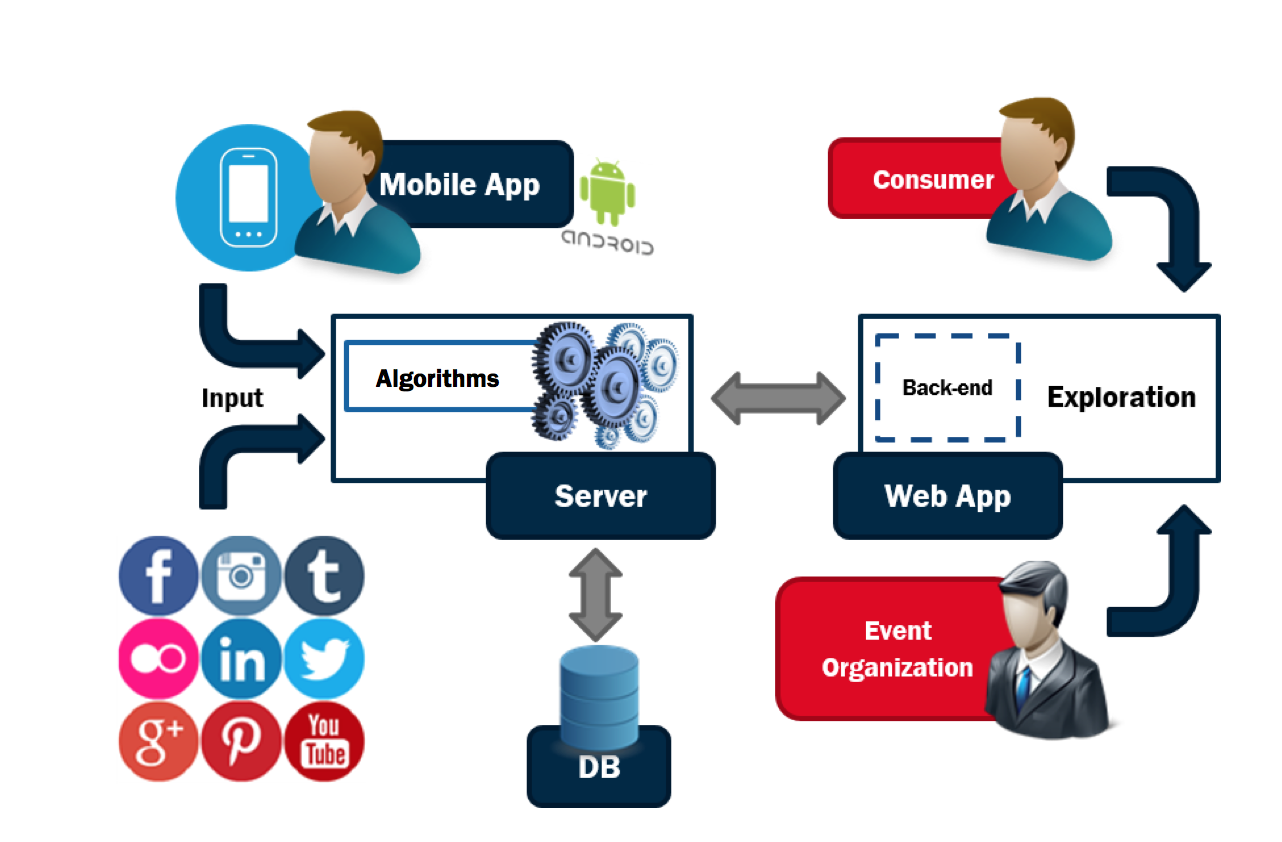
\epsfig{file=architecture.eps, width=2.72in}
	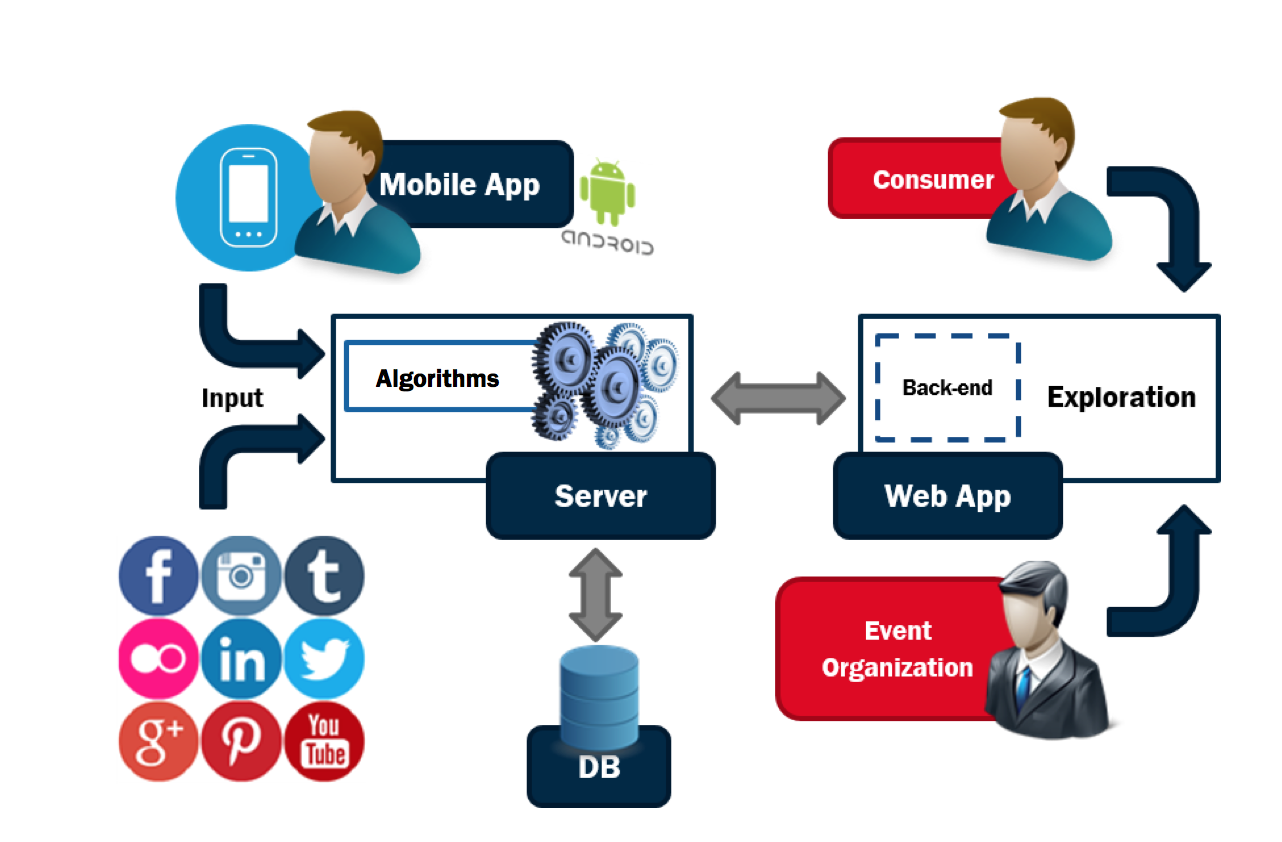
\includegraphics[width=0.7\linewidth]{architecture}
	\caption{The Social Picture's architecture.}
	\label{architecture}
\end{figure}
The collections can be explored from smartphones, tablet or desktop computers via a web application, which exhibits a range of filtering tools to better explore the huge amount of data (see Figure \ref{interface}).
%\subsubsection{Database}
%When a new image is added to the system, it is analysed by a set of algorithms with the aim to extract pre-defined features (both visual and textual), as well as semantic information. The image is collected, entered, processed and all the analysis results are stored in the Database. 
%\subsubsection{Mobile App}
%The mobile application allows users to upload their visual contributes to the event's collection. Other users can also contribute to the creation of the collection by posting their contents through the considered social netwoks, by adding a specific event's hashtag.
%\subsubsection{Web Application}
The web application shows different interfaces depending of the specific user and the event in which he has joined after an invitation from the event manager (the person who created the event). To join an event's collection, the user must upload at least one picture related to that event. Collections can be explored by several data visualization enviroments, which are selected by the event manager. Anyone registered to \textit{The Social Picture} can become event manager and start a social collection: this follows the ``prosumer'' paradigm, where the users are both producers and consumers of the service.
The developed framework is characterized by a modular architecture: new visualization interfaces, as well as new semantic filters can be independently created and futher added to the system. 
Thus, when an event manager creates a new collection, he is allowed to specify several options to customize the image gathering, the social analysis to be performed and the visualization tools for the users of that collection.
The event manager is also allowed to set a range of statistics, which will be available after the analysis of the collected images. These statistics helps organizators to extract useful social information from the crowdsourced pictures \cite{Milotta2016n544}. For example, what is the most popular artwork of a museum? What is the least considered? From which perspective these pictures were taken?
These information could be exploited, for example, to perform aimed investments. The system can suggest what is the better subject to use for the advertising campaign of the event, or which of the attractions it worth to mainly reproduce in the souvenir shop products, to support merchandising strategies. Feedback about what is the most interesting part (i.e., the most captured photo) of a landmark building can help on taking decisions about renovating some parts of the building rather than other as first investment, where the connotation of importance is achieved by the crowd who generated ``the social picture'' for that building by uploading related images.


\begin{figure*}[t]
	\centering
	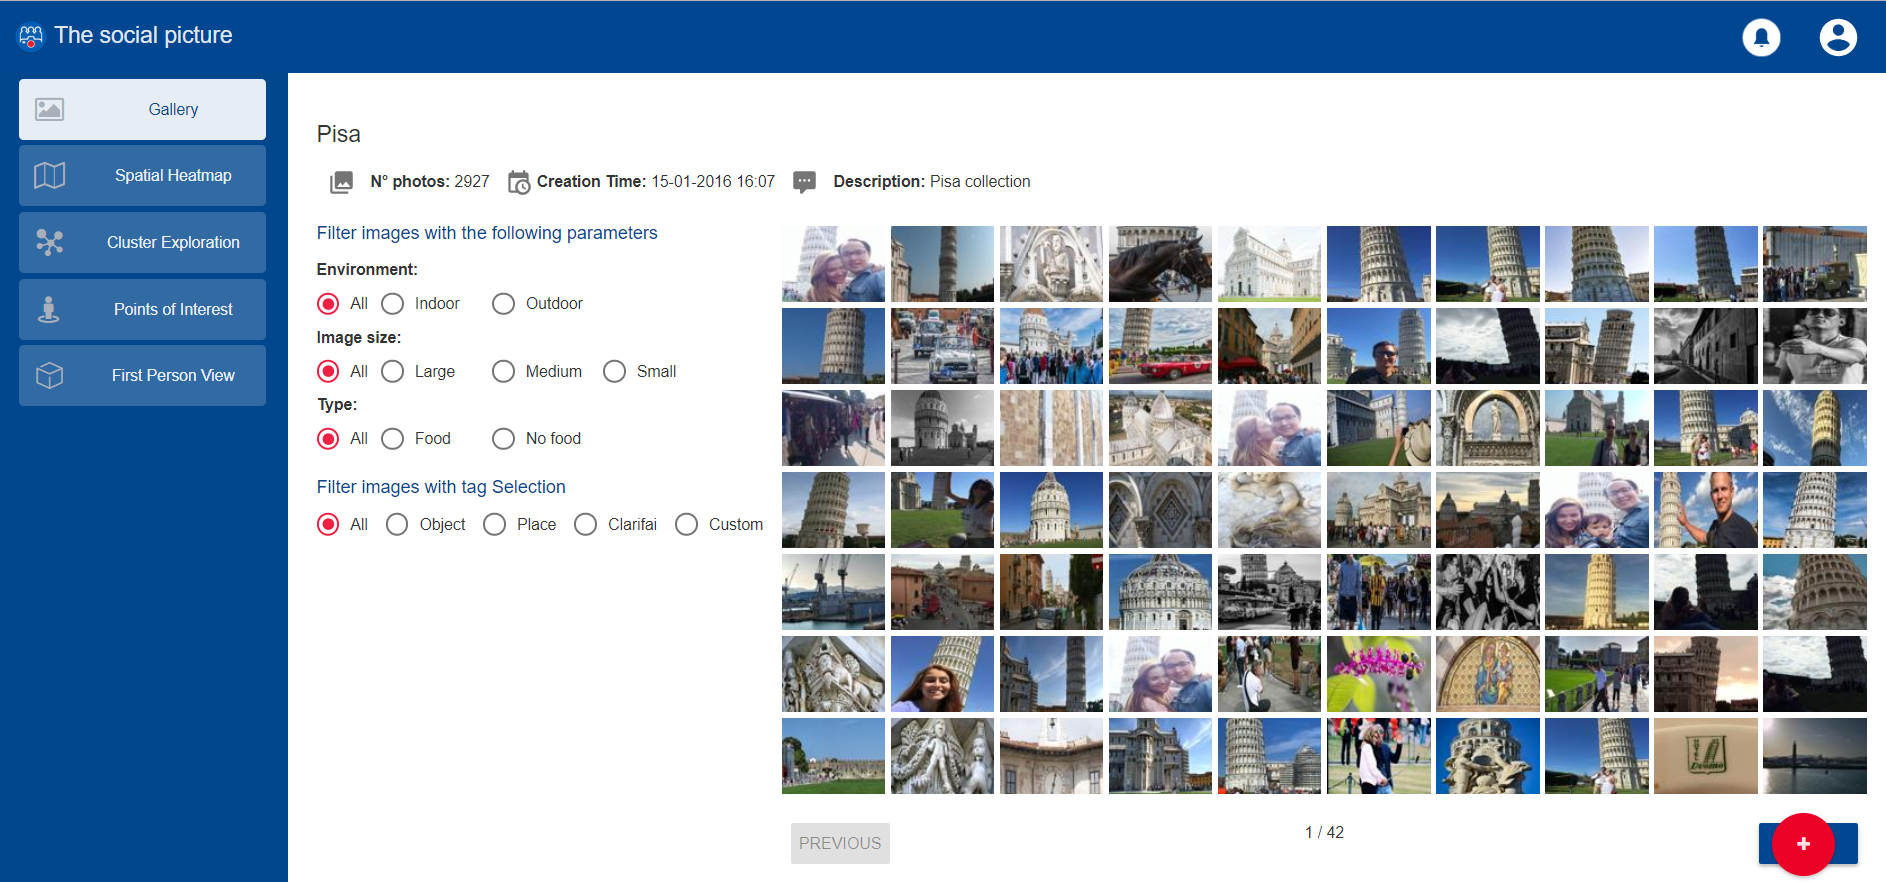
\includegraphics[width=1\linewidth]{gallery.png}
	\caption{Example of exploration interface. It is composed by three main areas: the gallery (right part) shows the collection's pictures according to the selected filters (middle) which allows the users to explore the collection. By selecting an image the system shows all the extracted information and the computed inferences (i.e., objects, places, similar images, if there is food, etc.). The filters allow to customize the set of images shown in the gallery. The menu (left) allows to select the visualization tool of the framework.}
	\label{interface}
\end{figure*}

%\begin{figure*}
%	\centering
%	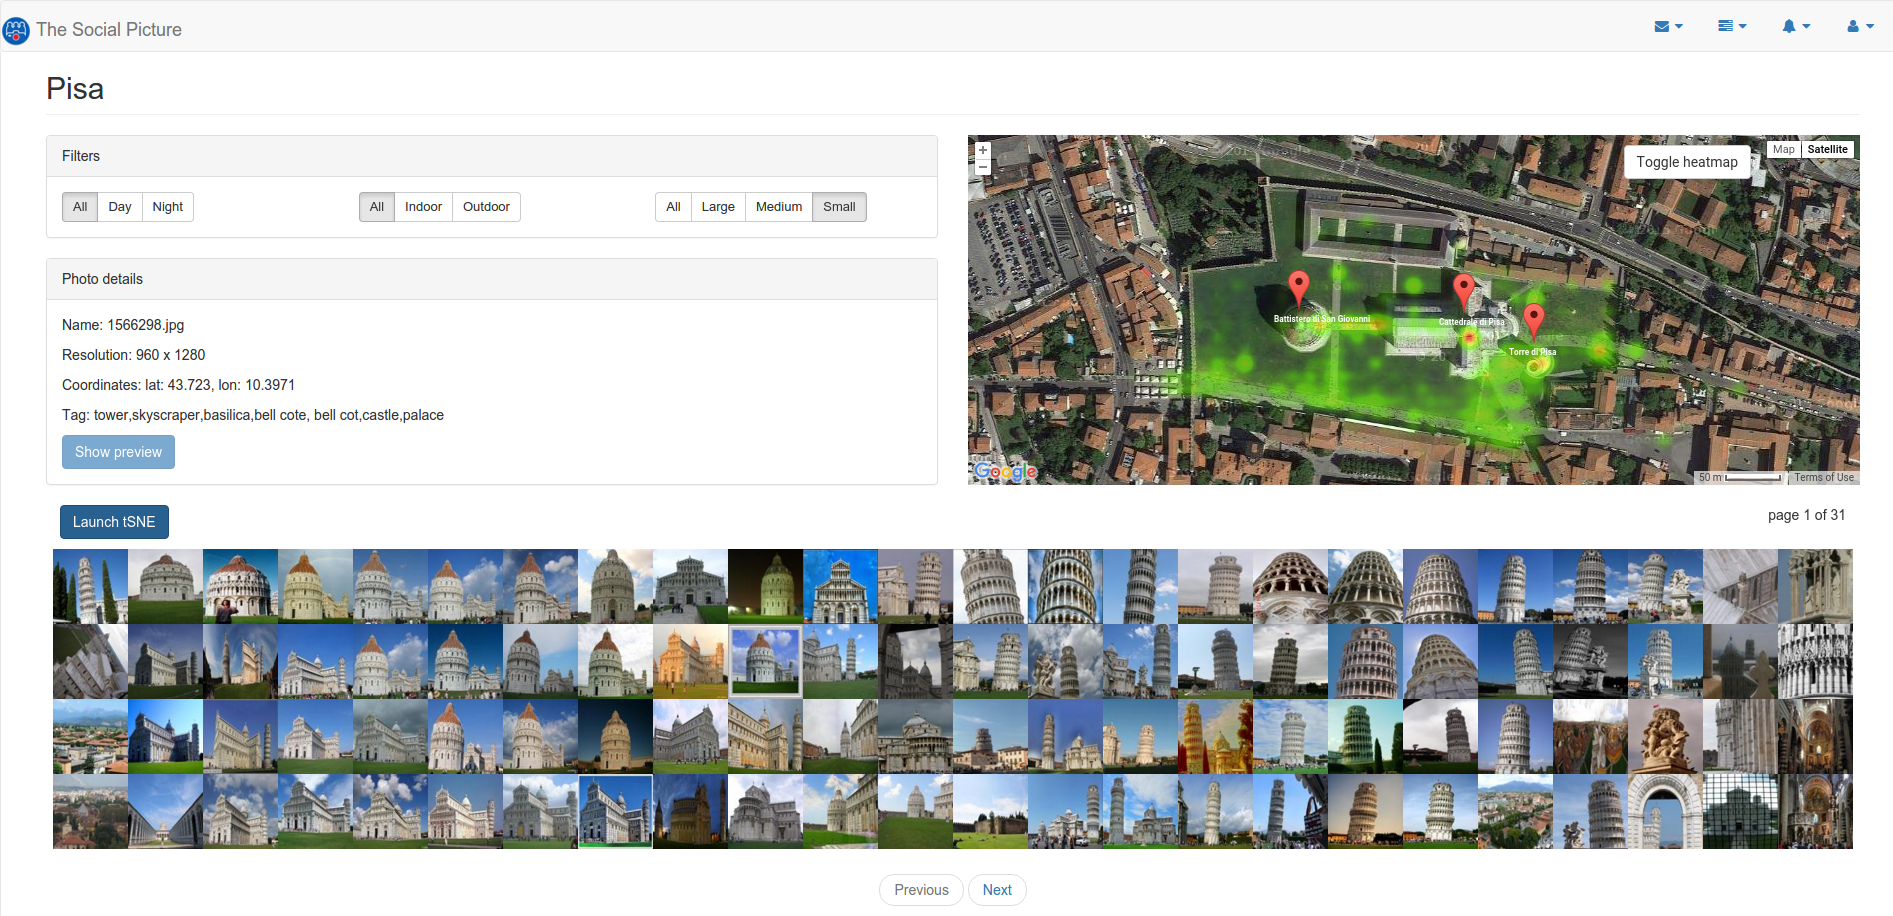
\includegraphics[width=1\linewidth]{interface01}
%	\caption{Example of exploration interface. It is composed by three main areas: the map area (upper-right) shows the positions where the images have been taken from. This give the positions of the users during the event and some hints about the most interesting parts of the site. The interaction with this map allows the users to know more details by selecting the images from their positions. The gallery (bottom) shows the collection's pictures organized by using t-SNE algorithm according to the selected filters and allows the users to explore the collection. The detail area (upper-left) shows the details of a picture selected from the gallery, and presents the available filters.
%		%TODO: CITARE IL TSNE SOLO PER LA VISUALIZZAZIONE AD HOC. NON NELLA DASHBOARD PRICIPALE.
%		From this interface, the user can launch the t-SNE algorithm on a customized set of images, apply one or more filters, and know more about the different statistics and inferences performed by the system.}
%	\label{interface}
%\end{figure*}
%\subsubsection{Analysis engine}
The several exploration tools are based on both visual and textual data. The system exploits information such as Exif data (camera model, geolocalization, acquisition details, and others) when available, and a number of ad hoc extracted visual features.

The visual analysis module of the system feds all the images to two different CNNs \cite{krizhevsky2012imagenet, zhou2014learning}, in order to extract the classification labels and an image representation. To attach semantic labels to the visual content of the images, we used \textit{AlexNet} \cite{krizhevsky2012imagenet} and \textit{Places205-AlexNet} \cite{zhou2014learning}.
The CNN used in \cite{krizhevsky2012imagenet} consist of seven internal layers with a final 1000-way softmax which produces a distribution over the 1000 predefined classes of the ImageNet dataset \cite{ILSVRC15}. We considered the feature activations induced at the last hidden layer, which consists of 4096 dimensional feature (fc-7 feature), as an image representation to be further used with t-SNE algorithm \cite{van2008visualizing} for visualization purposes. 
We also fed the images to the \textit{Places205-AlexNet} CNN \cite{zhou2014learning}. This CNN has the same architecture of \textit{AlexNet} CNN, but it is trained on 205 scene categories related to places learned by using the database \textit{Places205-AlexNet} composed by 2.5 million images.

%The results of the image evaluation by the above CNNs consist of the three classification predictions with the highest scores, given by each CNN, and the fc7 image representation.
\subsection{User experience}
An event manager (i.e., a user of \textit{The Social Picture} which starts a new collection) creates a new event by selecting among three possible type of event: public event (e.g., a concert), cultural heritage site (e.g., a museum) or private event (e.g., a wedding). The available event categorization can be extended to include other customized categories. We considered these three categories to better focus the aims of the specific analysis, and the inferred information that an organizator wants to extract.
The data gathering from users can be performed within a specific time window. The manager is allowed to control the image acquisition by selecting fine-grained criteria such as filtering media by hashtag, associated text or geolocalization distance.
After creating the event and its acquisition settings, the manager can select the statistics that the system have to compute by exploiting the collection of multimedia data gathered for that event.

The pictures can be grouped by hierarchical categories depending on the combination of two or more of the extracted visual features. %, which allow us to create several taxonomies in the image collection (panoramic pictures versus close-ups, natural versus artificial, indoor or outdoor, the presence or absence of crowds, selfies versus not selfies, and others).
Specific image categorizations help users to better handle huge amount of crowdsourced pictures, this kind of grouping can be exploited as a pre-processing before performing an image based visual search. Given a seed image, the system selects a set of similar pictures.
The system provides different exploration tools  %There is a tool for the exploration of outdoor collections such as cultural sites. % and whenever a large environment image can be considered as a reference for more detailed ones,
%One more tool 
that can be exploited to better navigate any huge image collection. These exploration tools together with other advanced tools are described in the next subsections.
A demonstration video of the framework is available at the following URL:
http://iplab.dmi.unict.it/TSP.

%\begin{figure}
%	\centering
%	%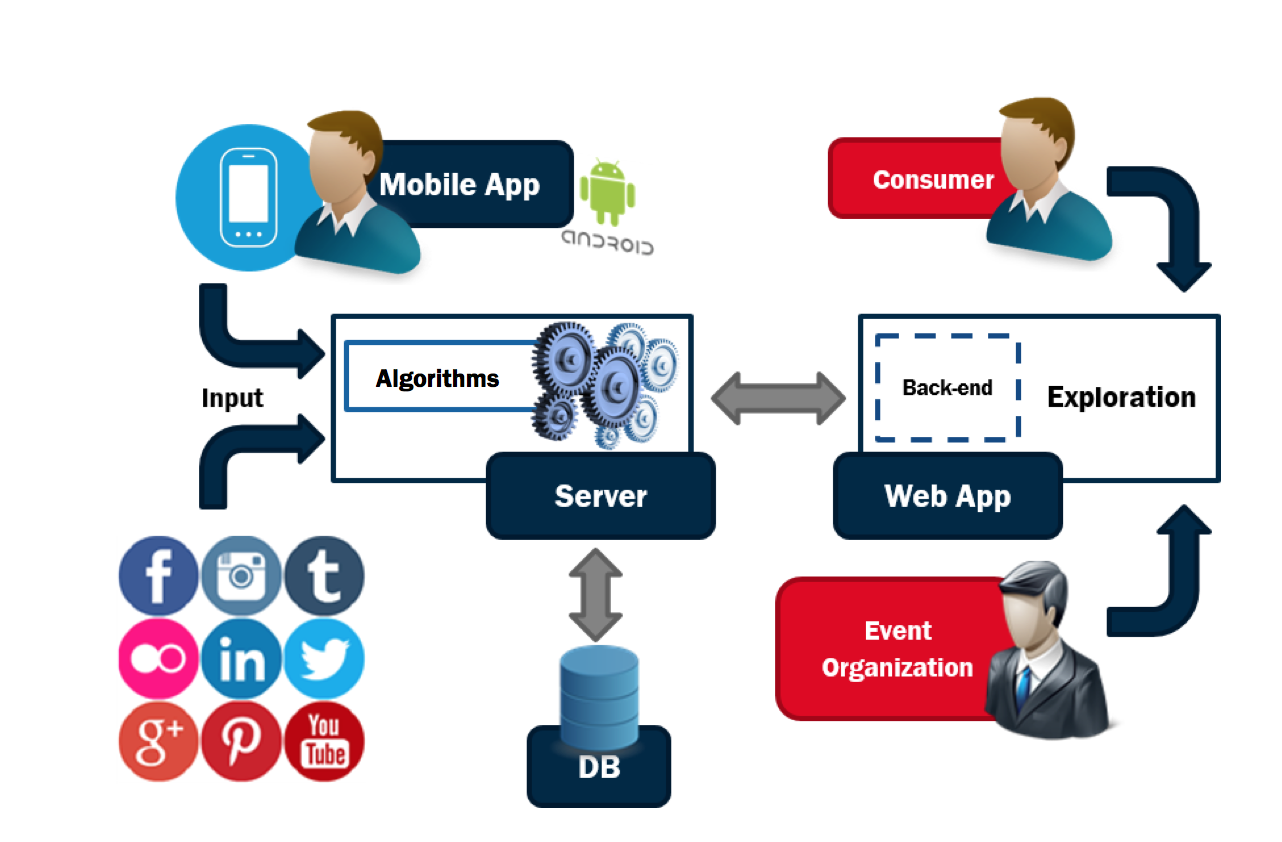
\epsfig{file=architecture.eps, width=2.72in}
%	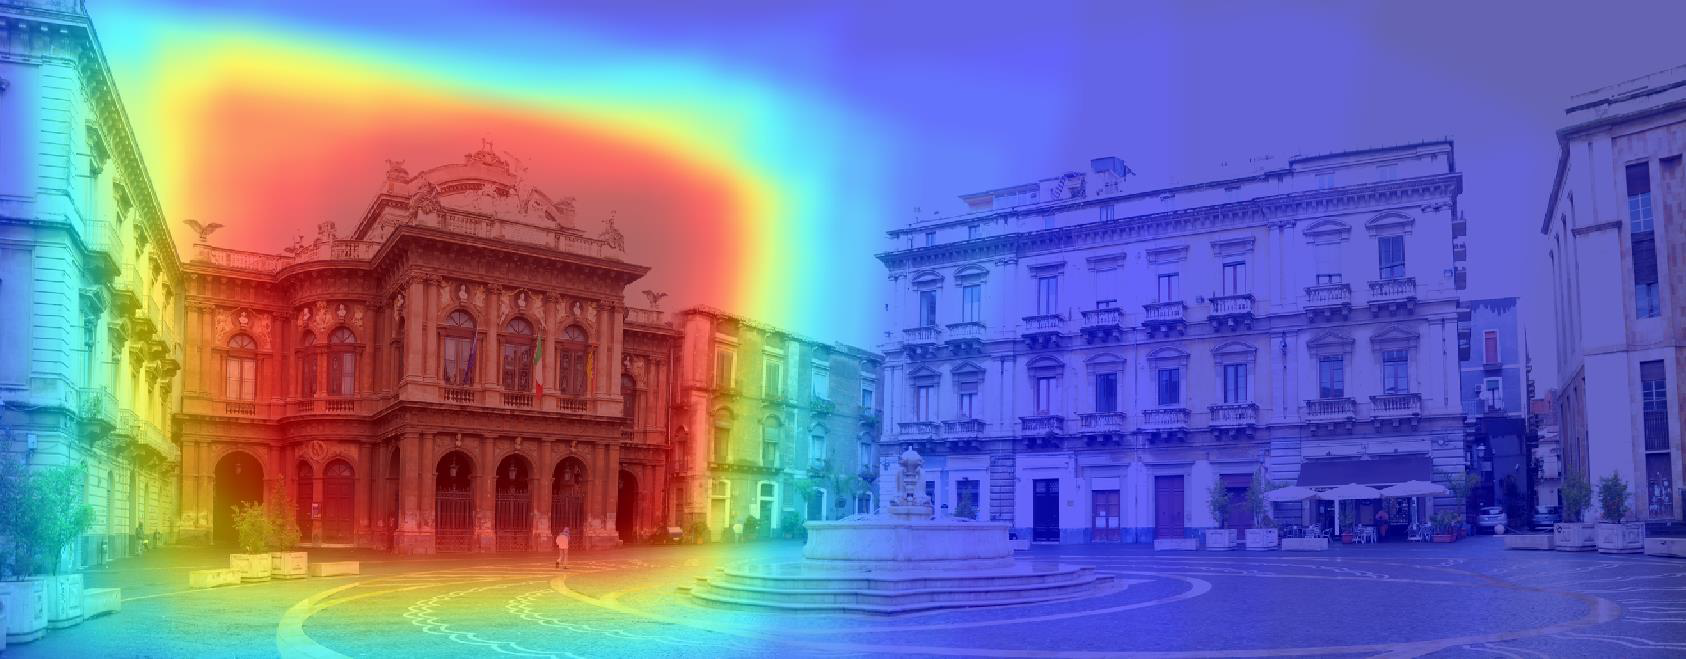
\includegraphics[width=1\linewidth]{heatmap}
%	\caption{Heatmap visualization.}
%	\label{heatmap}
%\end{figure}

\begin{figure*}
	\centering
	%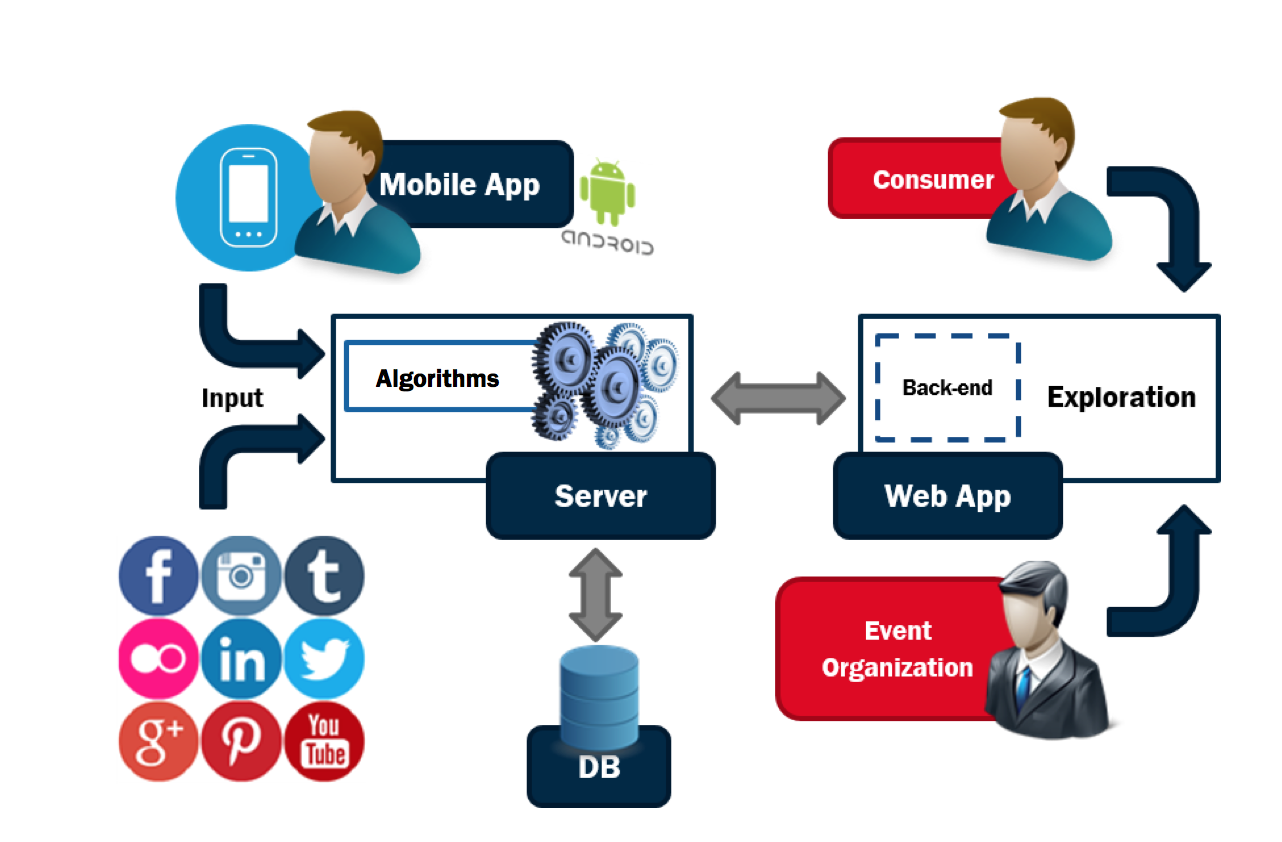
\epsfig{file=architecture.eps, width=2.72in}
	%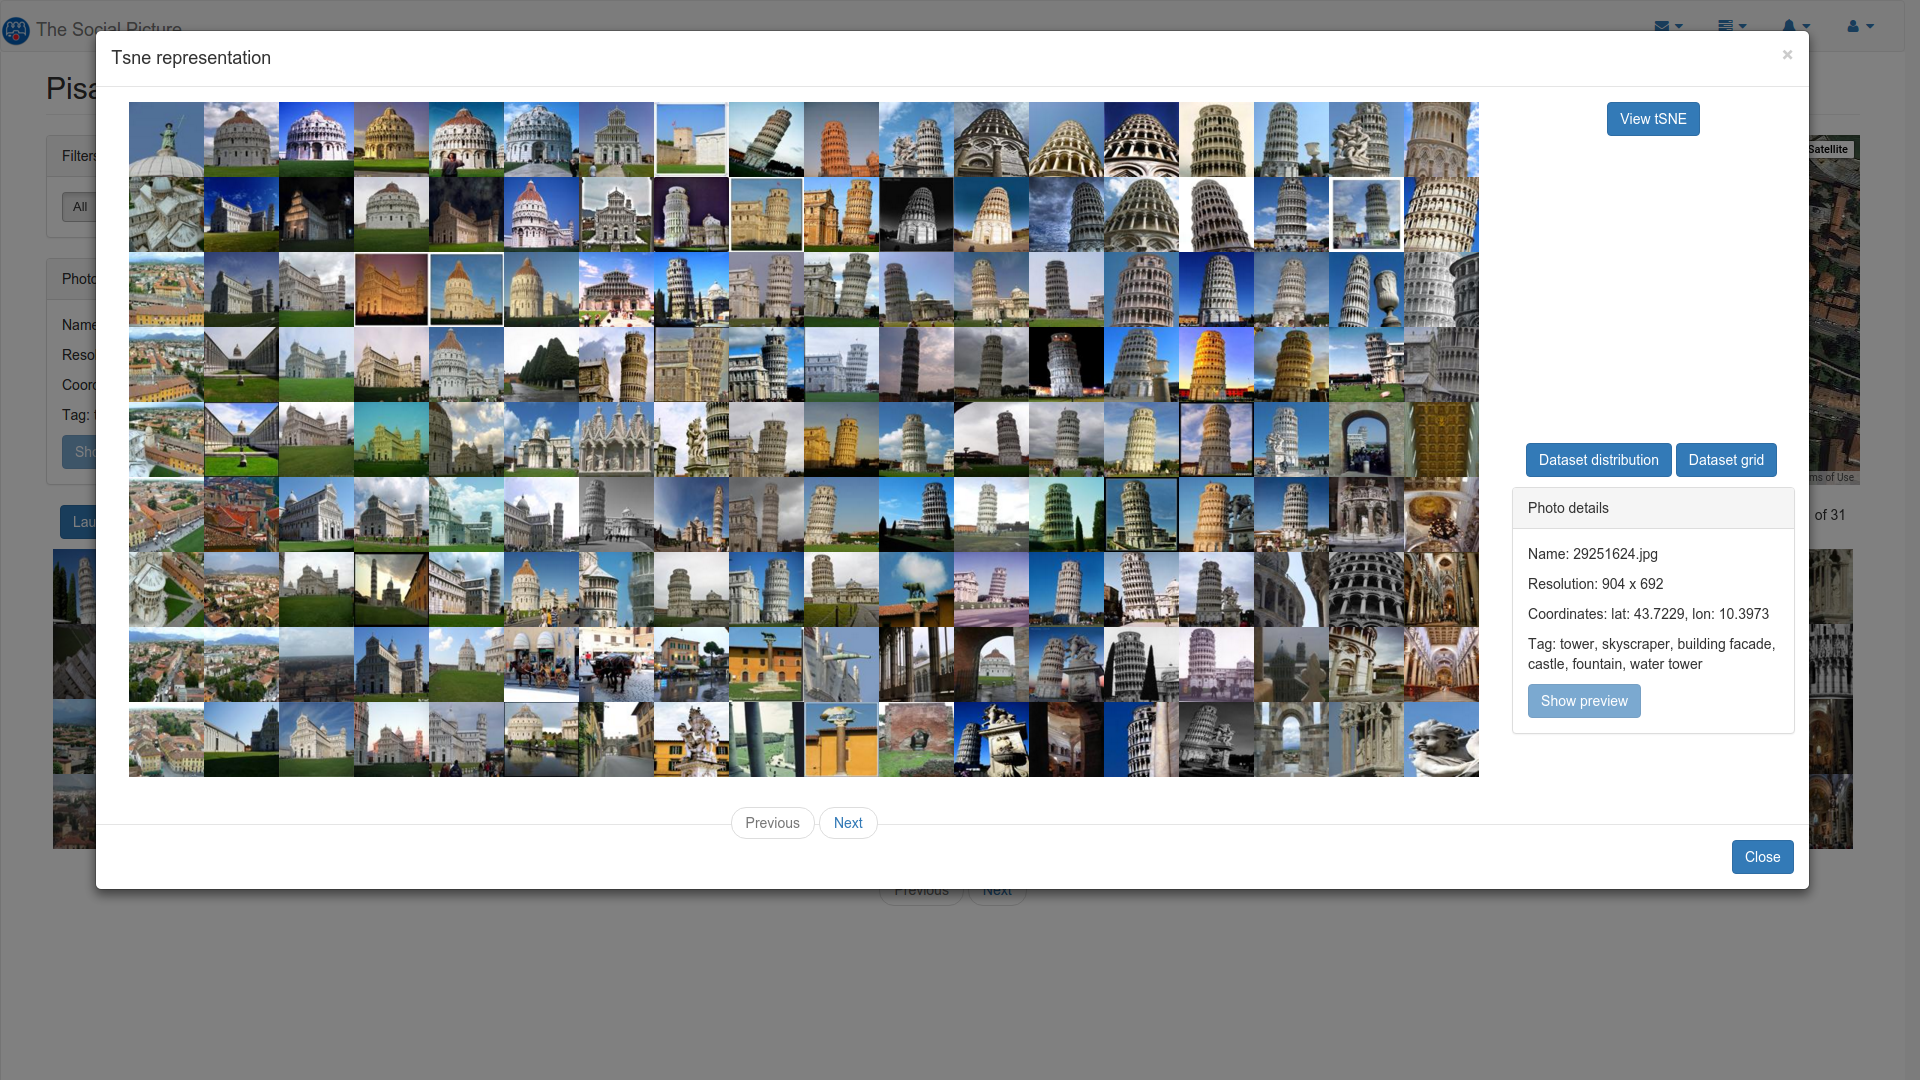
\includegraphics[width=1\linewidth]{gridtsne}
	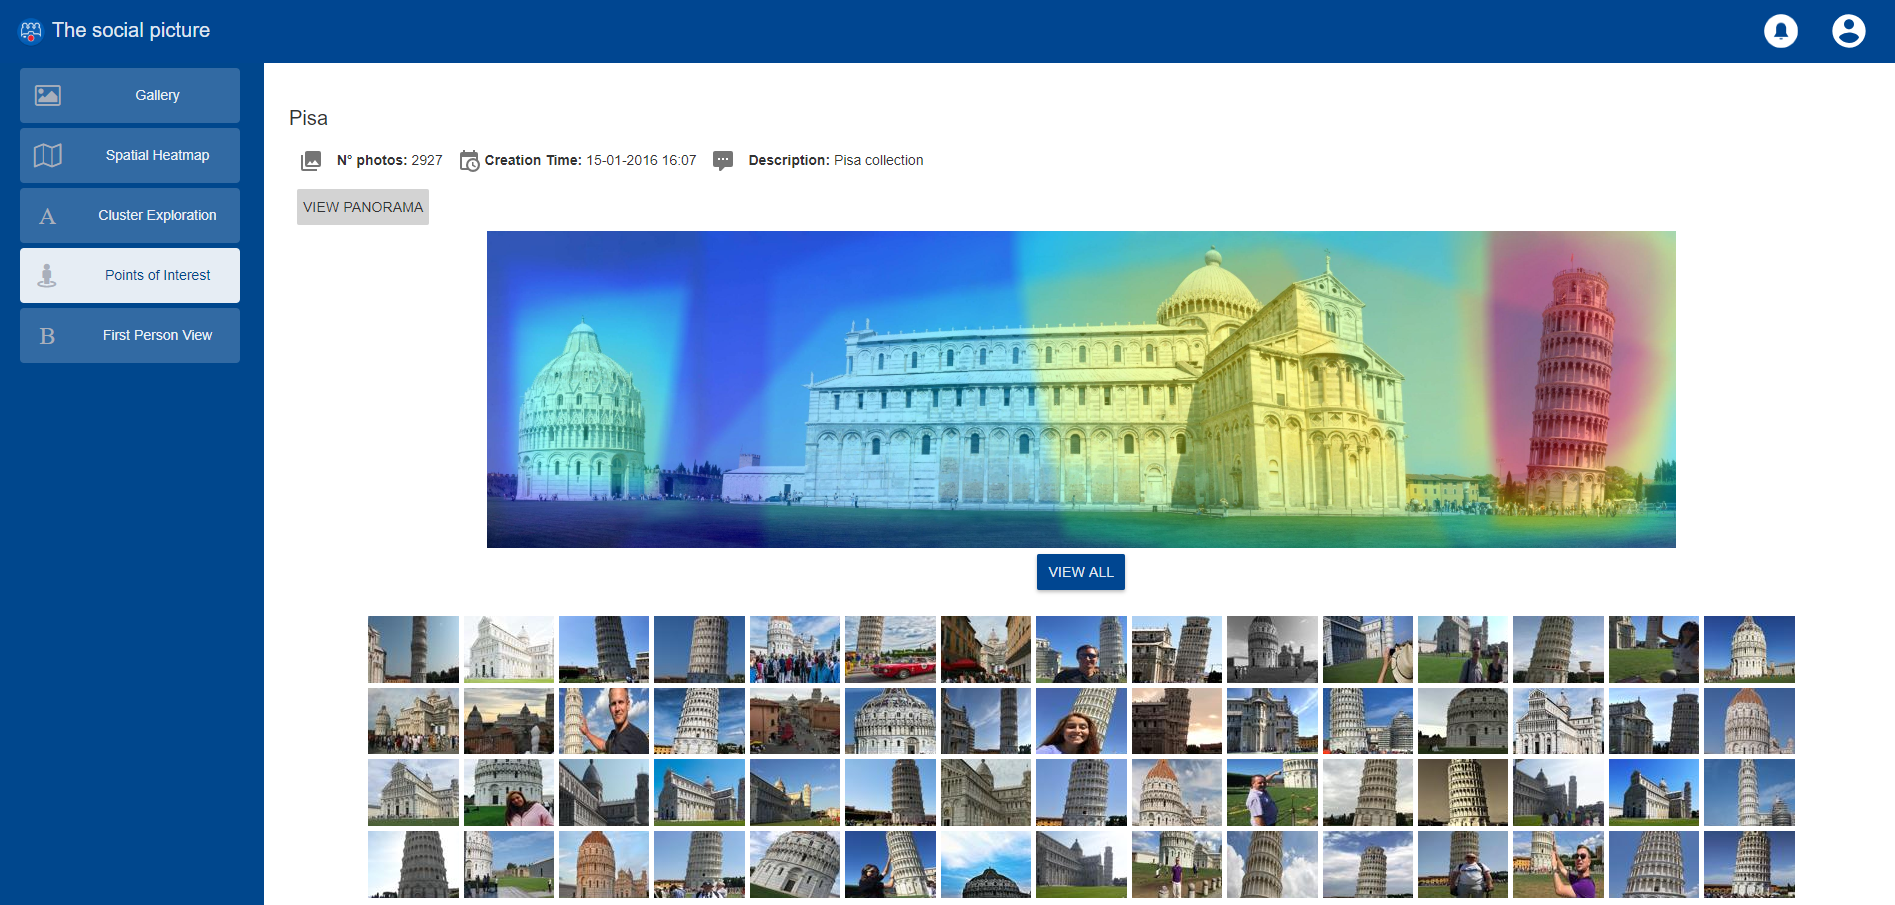
\includegraphics[width=1\linewidth]{heatGUI.png}
	\caption{heatmap exploration tool. By selecting a point in the heatmap, the system visualizes all the photos that contributed to that point in the bottom part of the interface.}
	\label{heatGUI}
\end{figure*}

\subsubsection{Heamap exploration}
In a cultural heritage site, people usually take pictures from different points of view and considering different details of parts related to famous and appreciated attractions and artworks. The heatmap exploration tool of \textit{The Social Picture} aims to infer the ``interest'' of people with respect to the different parts of a site. An example of heatmap generated from data in \textit{The Social Picture} is shown in Figure \ref{heatGUI}. Through this visualization tool, an organizer of a collection will be able to know which parts of the site captures people's interests.
On the other hand, users can explore the collection related to a site in a very simple and intuitive way. So, to highlight the ``interest'' of people related to parts of a site, the proposed system creates an heatmap by aligning images in \textit{The Social Picture} with respect to panoramic images of the site of interest~\cite{Mikulik2015}.

The heatmap is a visualization used to depict the intensity of images at spatial points. The heatmap consists of a colored overlay applied to the original image. Areas of higher intensity will be colored red, and areas of lower intensity will appear blue. The intensity of the heatmap is given by the number of collected pictures that contain that visual area.
By clicking on a point of the heatmap, the user can visualize the subject of images that contribuited to generate the map intensity at that point. This set of pictures can be further refined by selecting one of the images and asking the system to search similar pictures, or use the image subset as a starting point for further analysis. In other words, the heatmap visualization gives the possibility to understand the behaviour of the people, especially if it is combined with the information coming from the geolocation of the devices in the instant of the photos creation. Also it can be considered as a powerful and intuitive image retrieval tool for the collections related to cultural heritage sites.
\begin{figure*}
	\centering
	%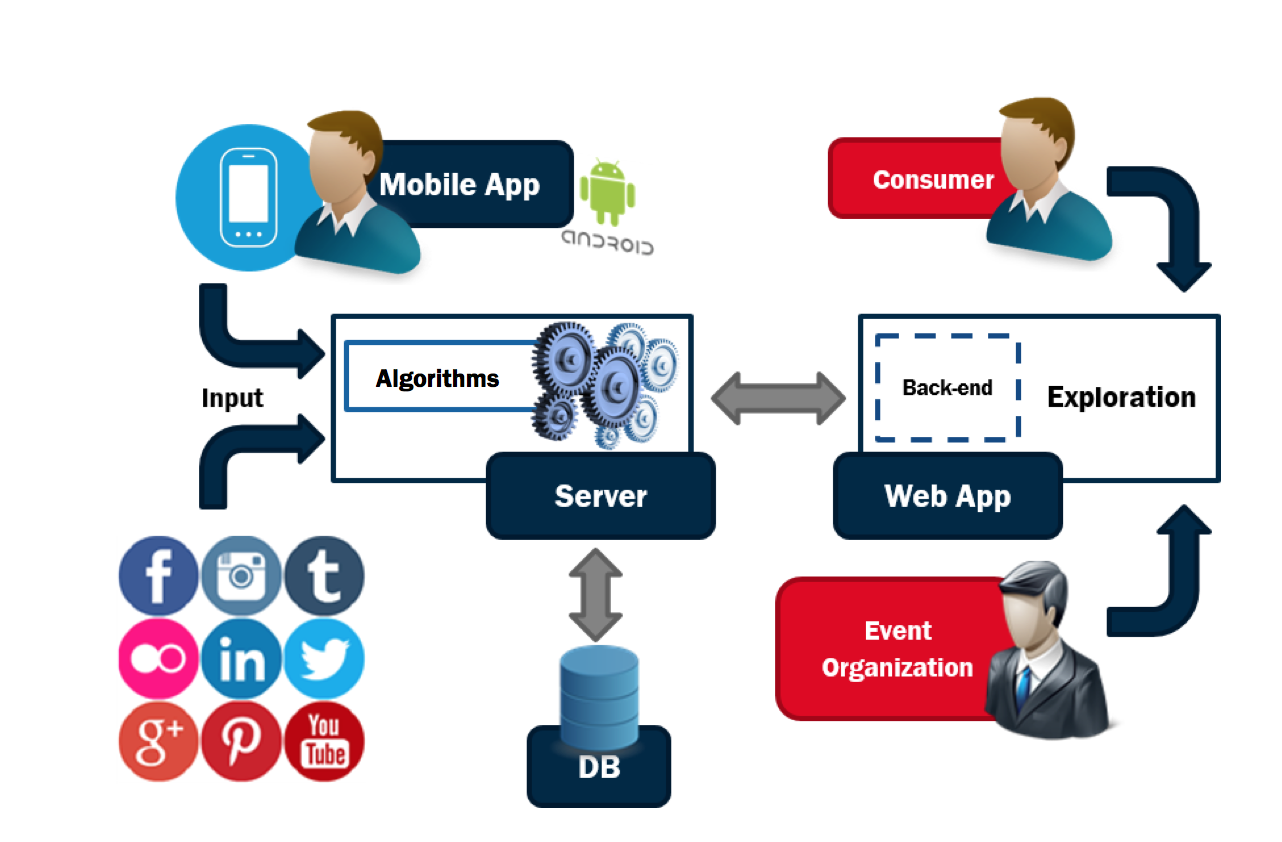
\epsfig{file=architecture.eps, width=2.72in}
	%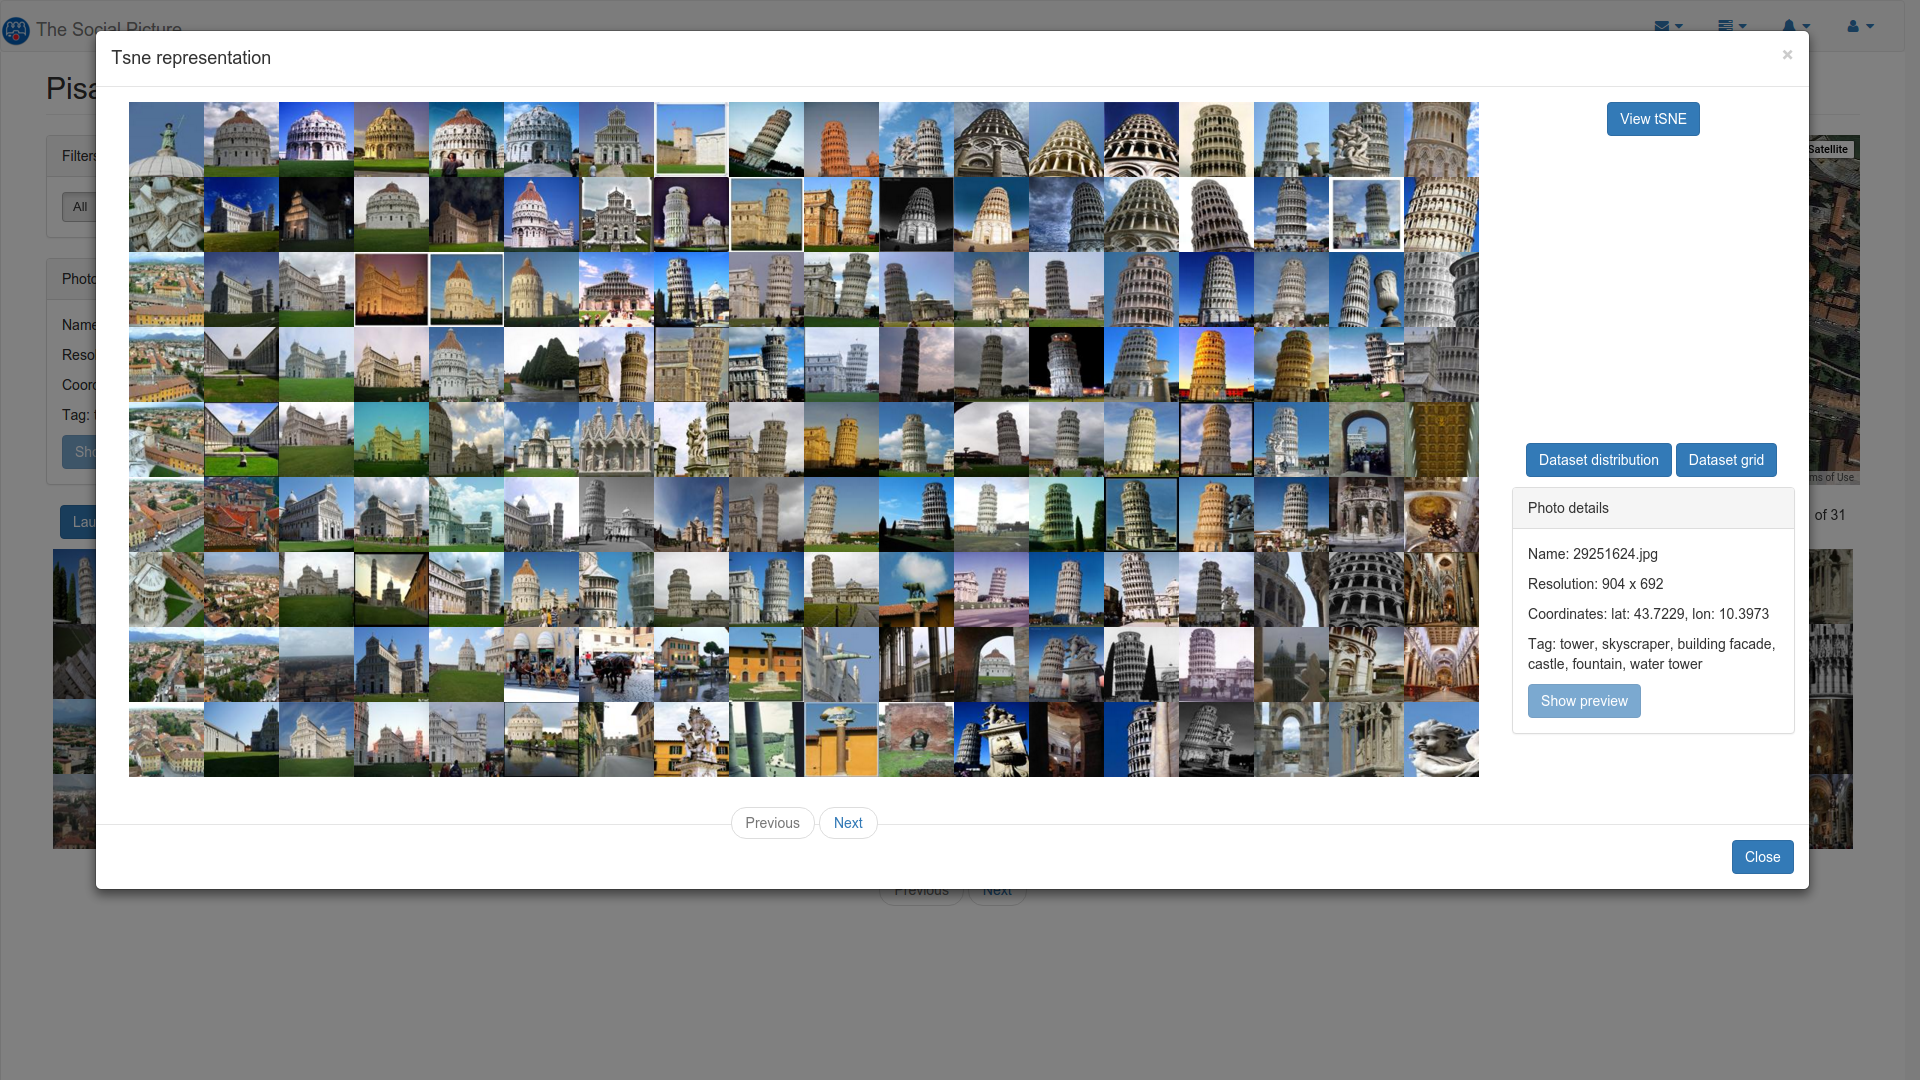
\includegraphics[width=1\linewidth]{gridtsne}
	\includegraphics[width=1\linewidth]{3Dmap.png}
	\caption{3D sparse reconstruction of a cultural heritage site based on the photos of the collecction. Each point in the 3D space is estimated by considering the projections of the images depicting that part of the scene.}
	\label{3Dmap}
\end{figure*}

\paragraph{3D Reconstruction}
Starting from VSFM (Visual Structure From Motion)~\cite{wu2013towards}, we are able to compute a 3D sparse reconstruction of large photos collections. The models are augmented with colors for vertices, related to the frequency of been acquired in a photo, colors for cameras, related to the number of visual features acquired by each photo, and with a plane which show the spatial density of contributing users. We embedded in TSP the models through a 3D web viewer allowing the users to browse the 3D sparse reconstructed models gaining a cue about what are the points of view and the subjects preferred by users when take photos. %Moreover, the models in the 3D web viewer can also be browsed through Leap Motion system, an intuitive and fast interactive system.
\vspace{-0.2cm}



\subsubsection{Embedding Exploration}
We exploit the fc7 feature extracted with the \textit{AlexNet} architecture~\cite{krizhevsky2012imagenet} for each image and use the t-SNE embedding algorithm~\cite{van2008visualizing} to compute a 2D embedding that respects the pairwise distances between visual features.
The t-SNE (t-Distribuited Stochastic Neighbour Embedding) is a technique for feature space dimensionality reduction that is particularly well suited for the visualization of high dimensional image datasets.
In Figure~\ref{gridtsne} the images are first assigned to a 2D position in the embedding space by means of the t-SNE algorithm, then we forced the images to fit a grid layout for a better visualization. Note that images with the same subject are automatically arranged nearby (see Figure \ref{gridtsne}). Moreover, the system arranges very close those images which are not the same but have a similar visual content. It is also important to highlight that the employed CNN~\cite{krizhevsky2012imagenet} has been trained using a different dataset concerning 1000 classes of objects, but the fc7 features resulted expressive and representative enough to be applied successfully to a generic event collection.
\begin{figure*}
	\centering
	%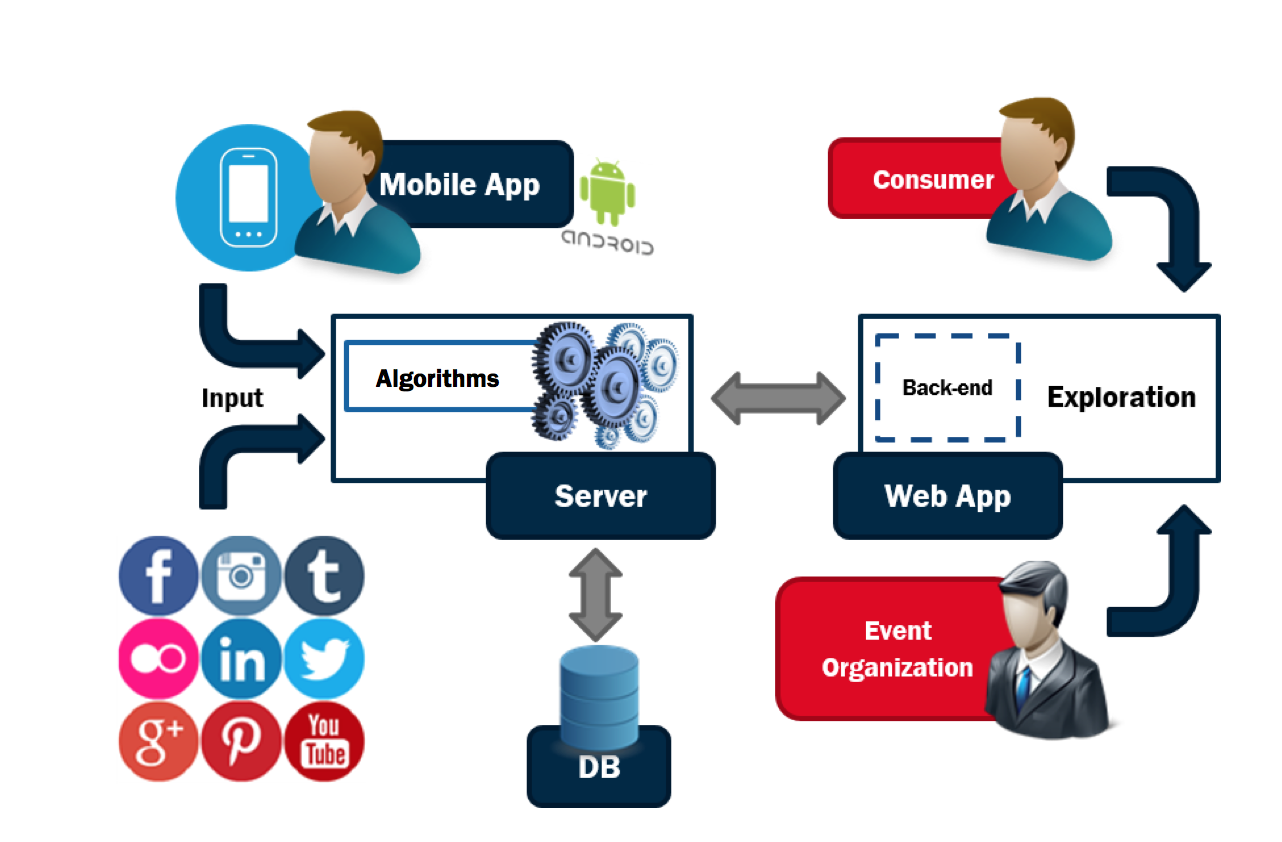
\epsfig{file=architecture.eps, width=2.72in}
	%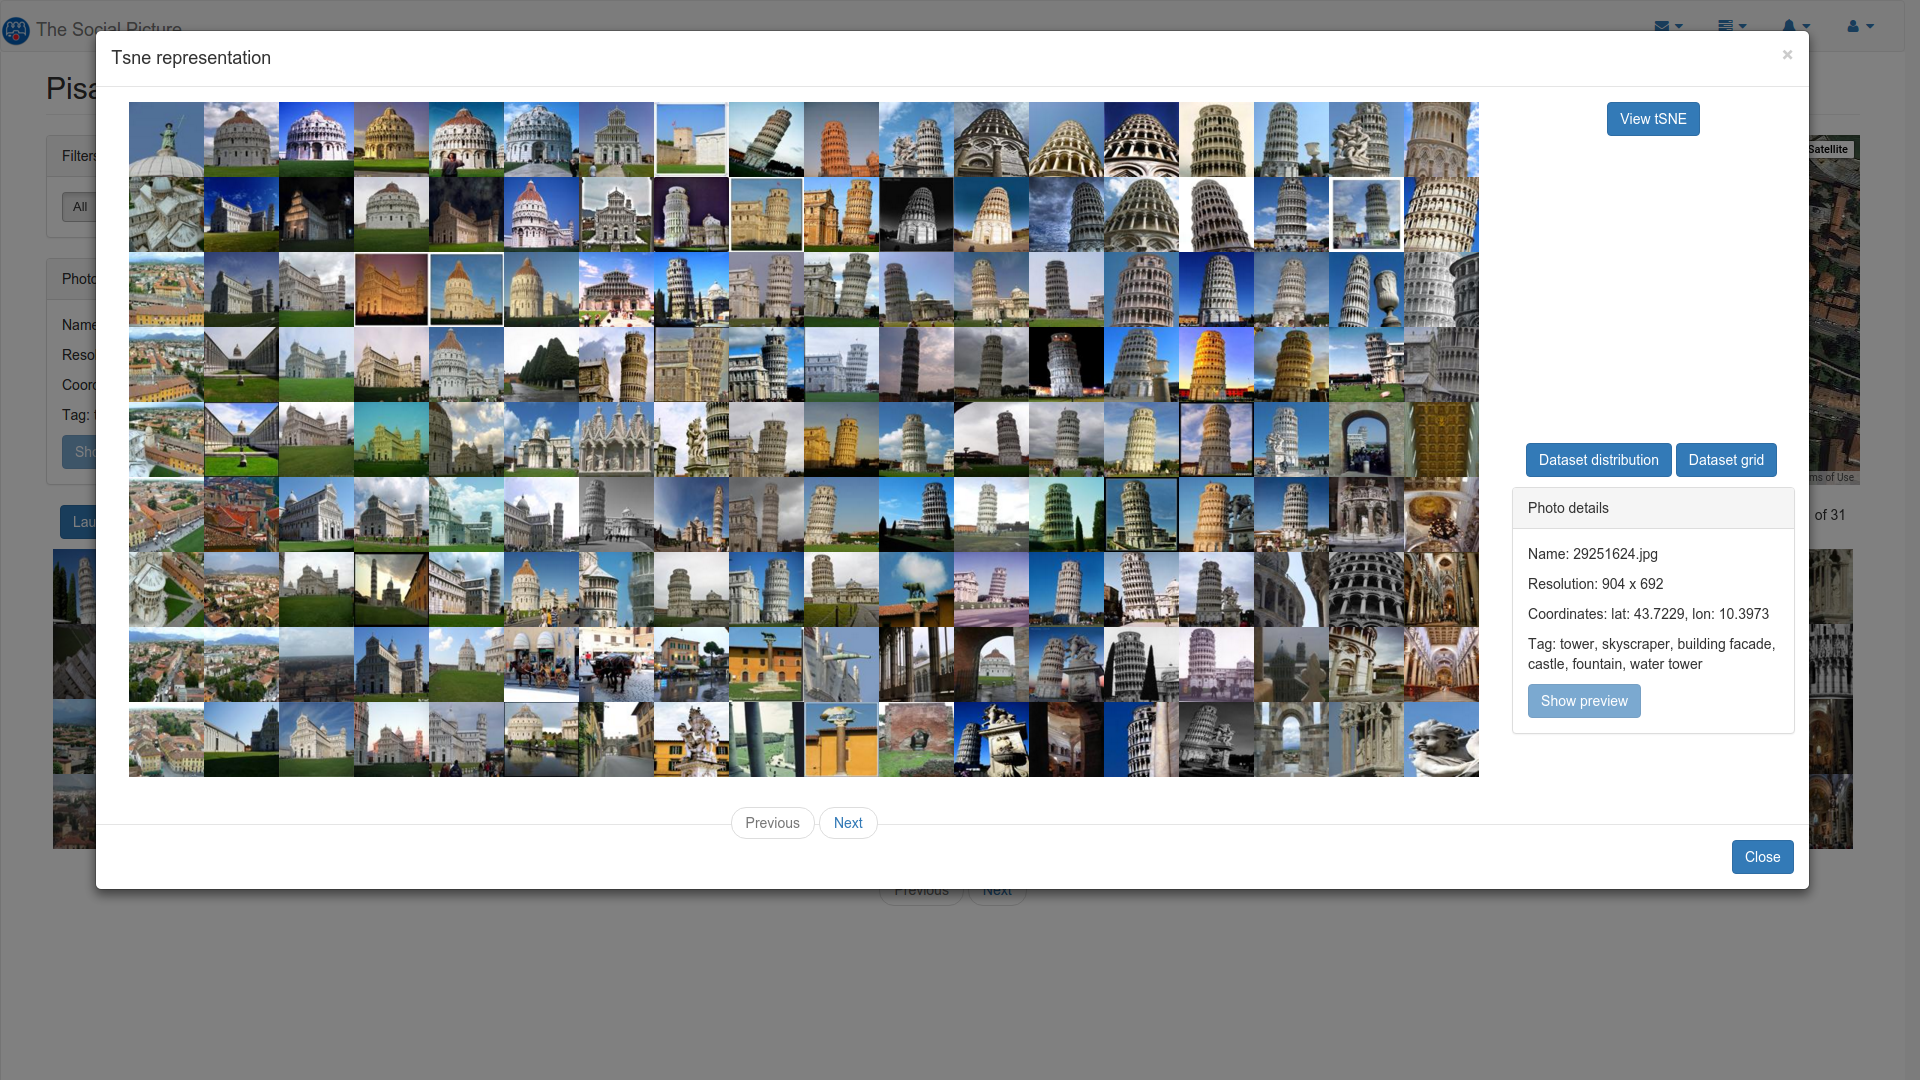
\includegraphics[width=1\linewidth]{gridtsne}
	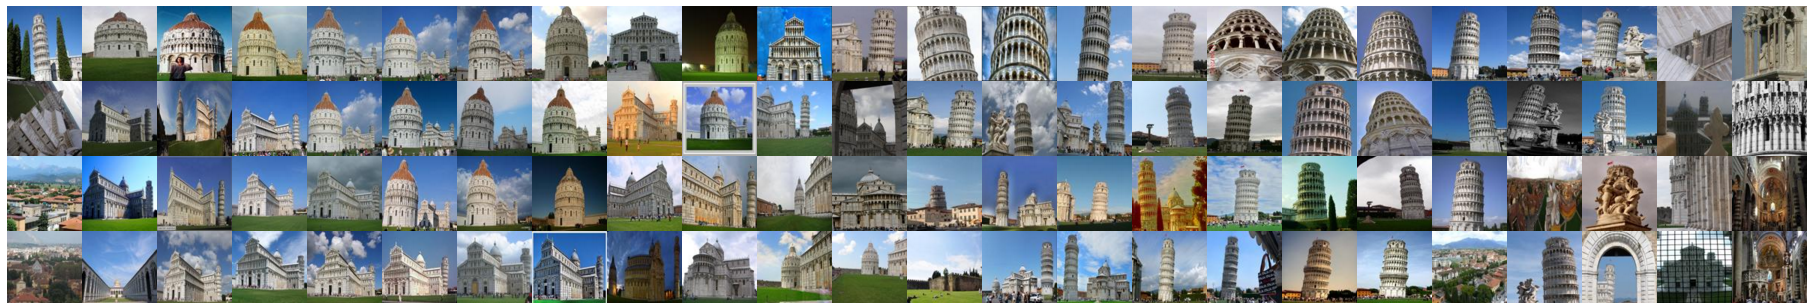
\includegraphics[width=1\linewidth]{tsneFixed.png}
	\caption{t-SNE visualization, the images are forced to fit a grid layout. Images of an event are automatically organized by visual content. Images close in the 2D space of the visualization tool are also close in terms of visual content.}
	\label{gridtsne}
\end{figure*}
\begin{figure*}
	\centering
	%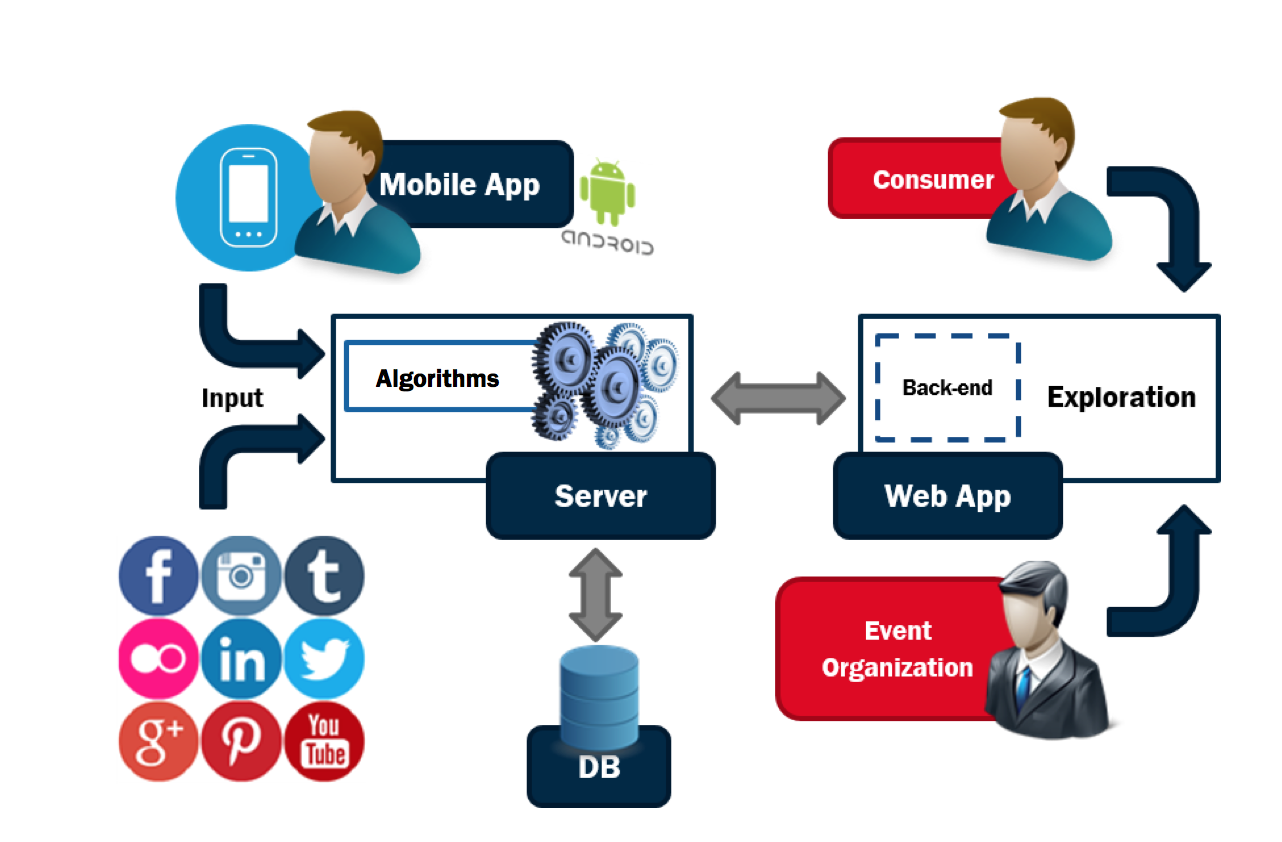
\epsfig{file=architecture.eps, width=2.72in}
	%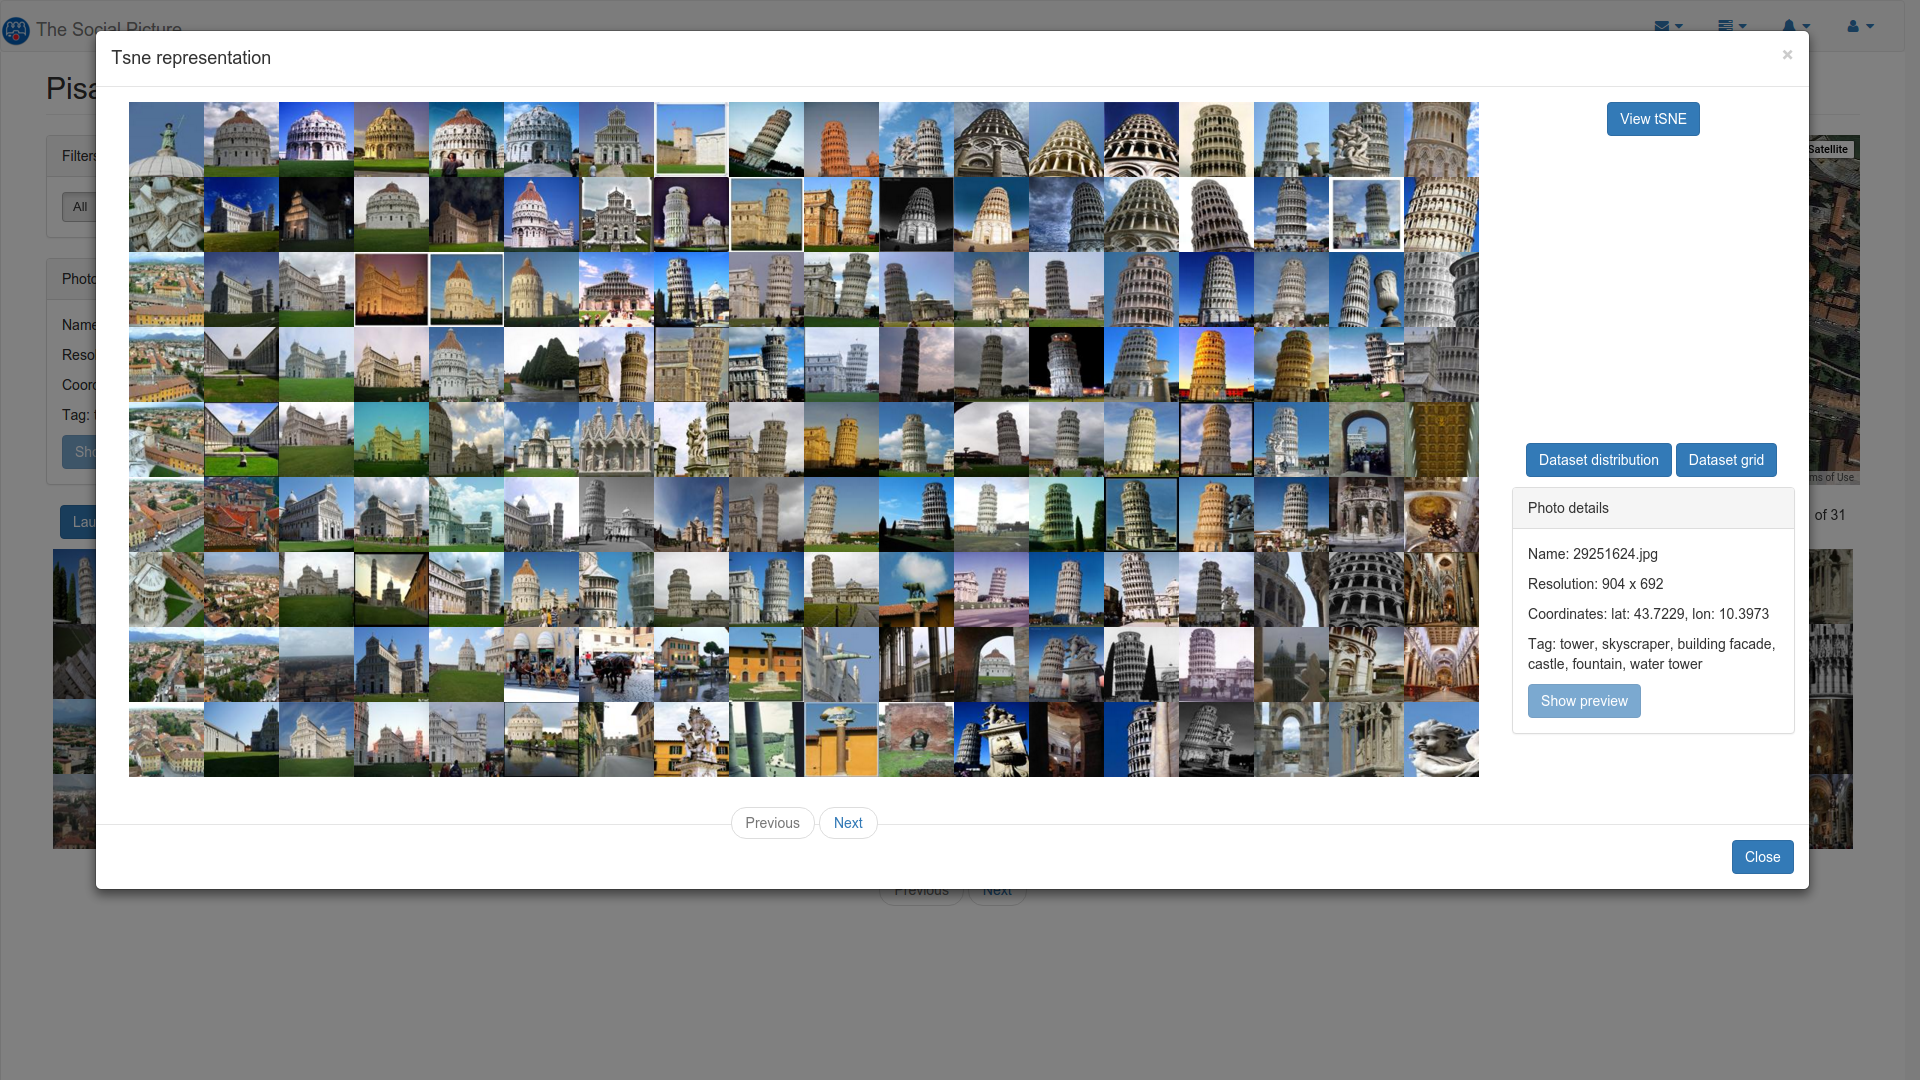
\includegraphics[width=1\linewidth]{gridtsne}
	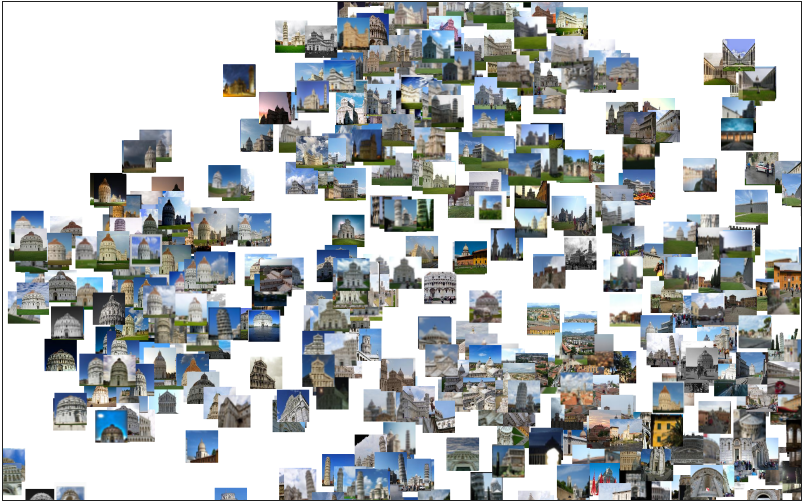
\includegraphics[width=1\linewidth]{tsne.png}
	\caption{photos embedding based on the t-SNE coordinates.}
	\label{tsne}
\end{figure*}

Another exploration tool allows users to visualize the result of t-SNE embedding without using the grid layout. Images related to similar subjects will be clustered implicitly, without any semantic hints.
This allow the exploration of the different sets of images composing the collection. For instance, photos of the same building but different lighting or weather conditions are arranged nearby, depending on their pairwise similarity. Photos of the same building but from different point of views are arranged in further sub-groups. Indeed, depending on the analysed photos, this automatic grouping can have different level of granularity. These automatically generated groups can be exploited to select the \virgolette{best} photo among the cluster of photos related to the same scene, or remove duplicates in the collection as instance.
When we display a set of images using their embedded locations computed by t-SNE, they may overlap one each other. Especially if there are many similar images. For this reason, this interface provides a set of tools to help the user's navigation.
With this exploration tool, the user can apply a translation or a zooming to all the viewed images, just clicking and dragging the mouse along the desired direction and by using the scroll wheel respectively. This helps the user to better explore the image distribution in a custom level of detail.
%A number of tools enable users to fine-tune the spread of images along X and Y axis, and the zooming effect. These parameters can be used to transform the distribution of the embedded images, and adapt the effect of the mouse commands. For example, if the user fix an upper bound for the zoom effect, when this limit is reached the scrool wheel of the mouse has the effect of separating the images according to the amout of the rotation.
%Furthermore, the user can choose a subset of images and compute the t-SNE embedding of them directly on the browser (see Figure \ref{gridtsne}).% This tool has been developed by using the \textit{tsnejs} Javascript library by Andrej Karpathy.


\paragraph{Hierarchical t-SNE}
The first implementation of the t-SNE exploration tool in~\cite{battiato2016social} was unable to scale with the number of the collections' images. We further extended this tool by implementing an hierarchical version of the t-SNE embedding which allows to explore picture collections without limits on the amount of processed pictures. 
This helps the user to better explore the image distribution in a custom level of detail. Furthermore, the user can choose a subset of images and compute the t-SNE embedding of them directly on the browser. % This tool has been developed by using the \textit{tsnejs} Javascript library by Andrej Karpathy.

\begin{figure*}
	\centering
	%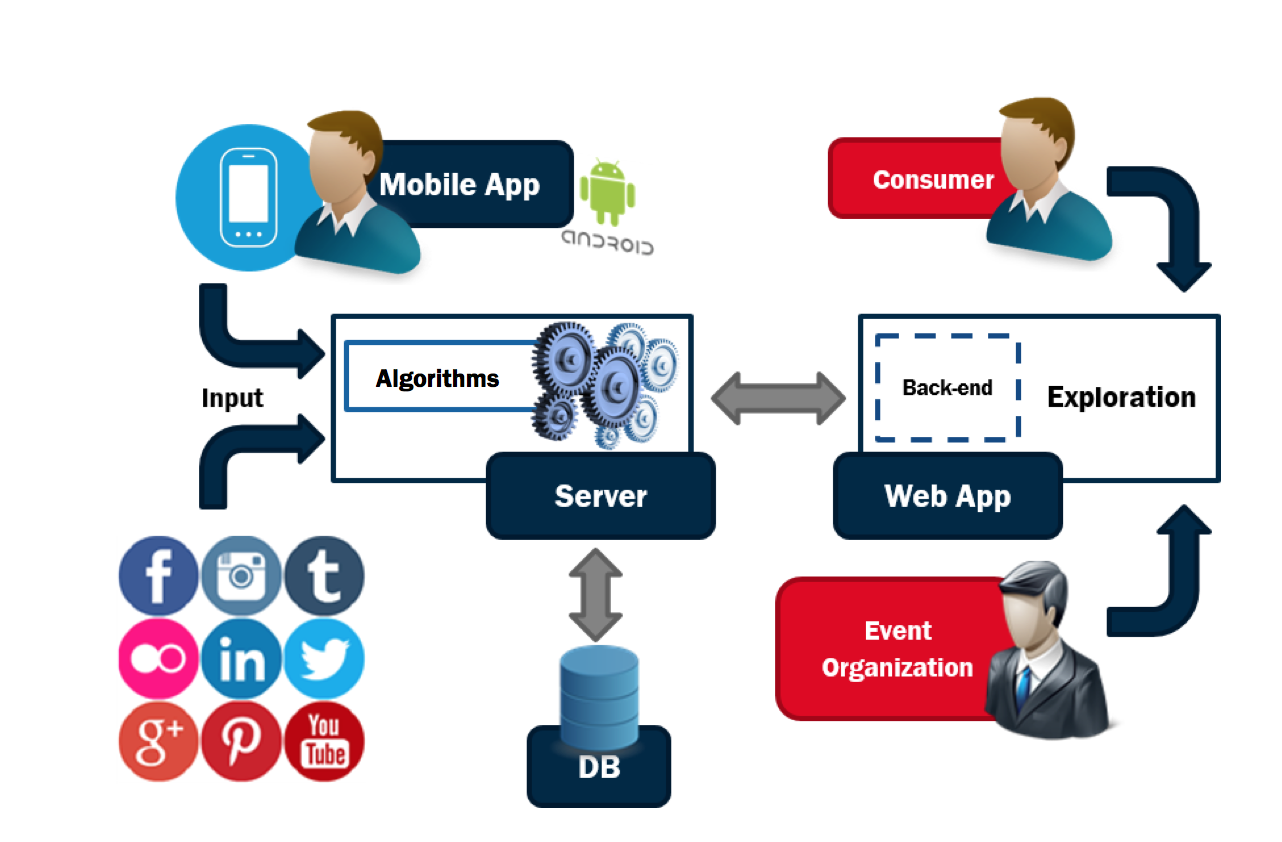
\epsfig{file=architecture.eps, width=2.72in}
	%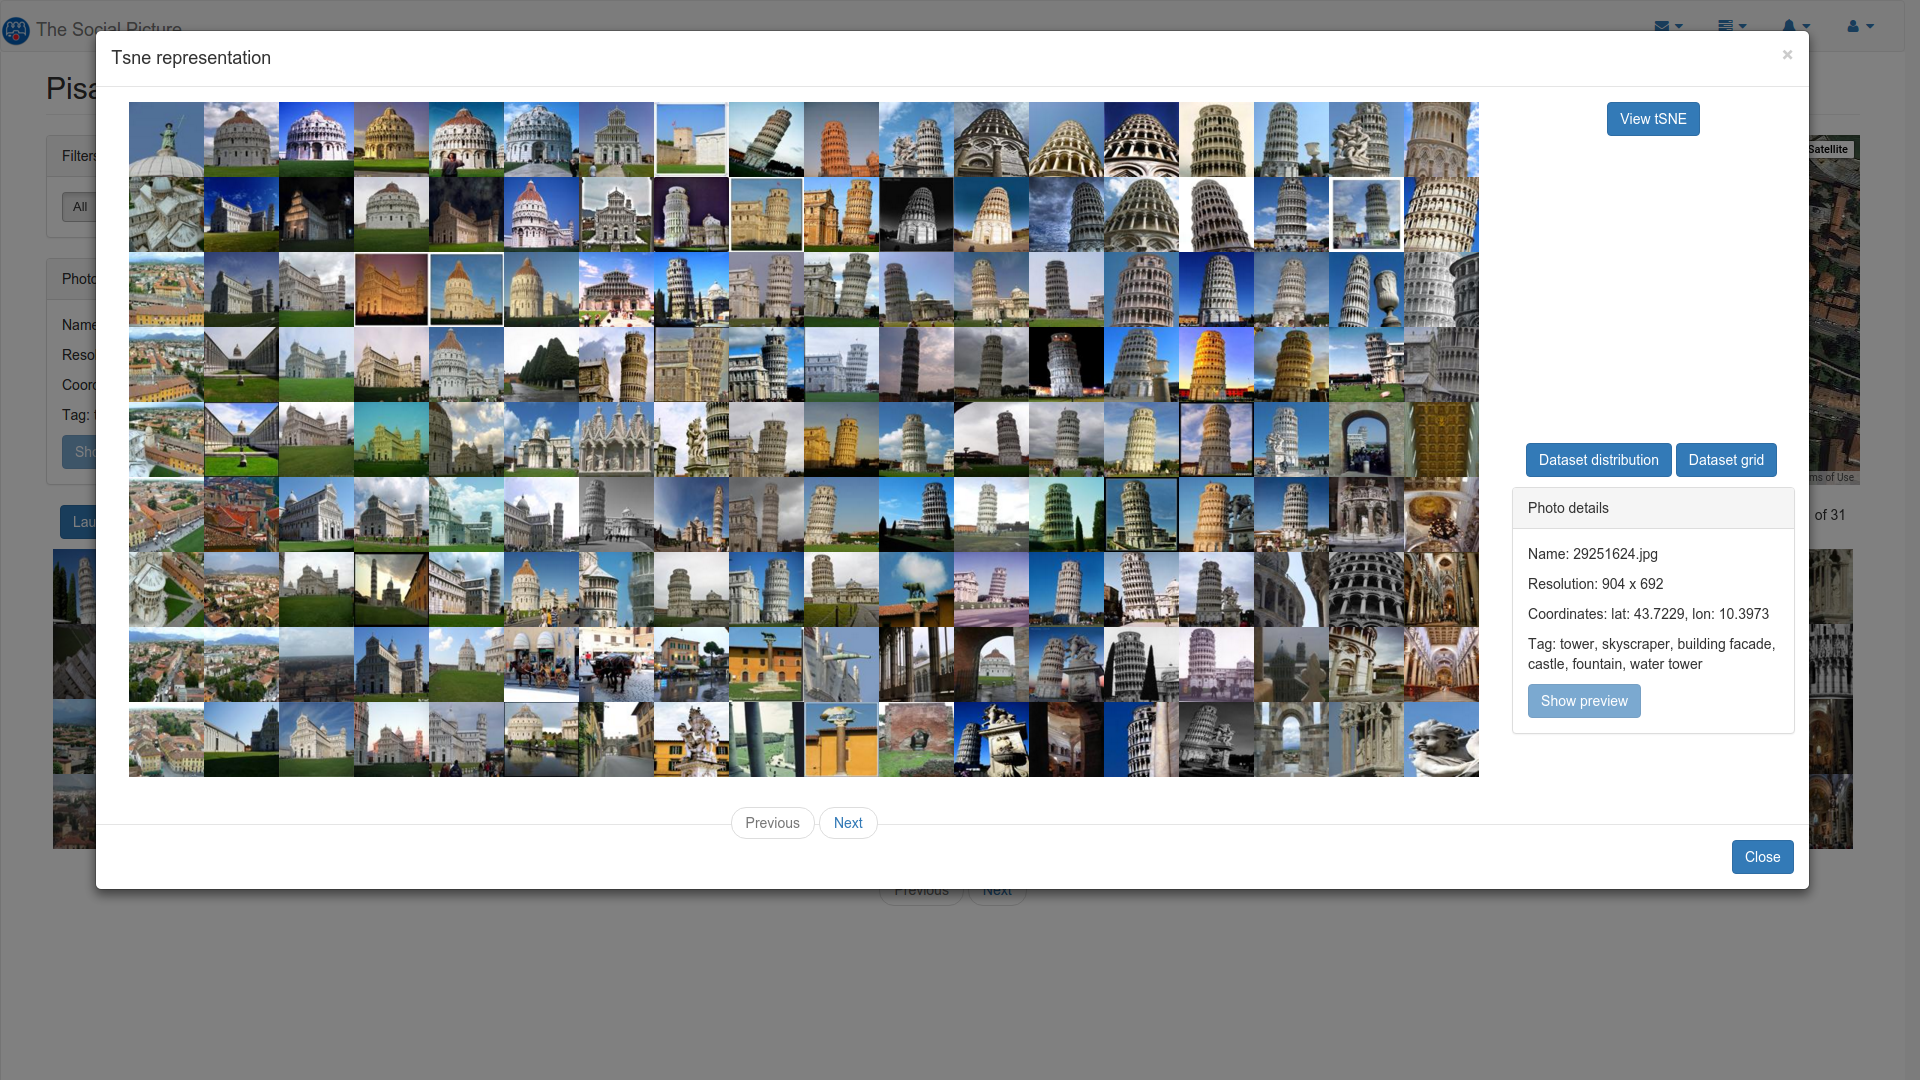
\includegraphics[width=1\linewidth]{gridtsne}
	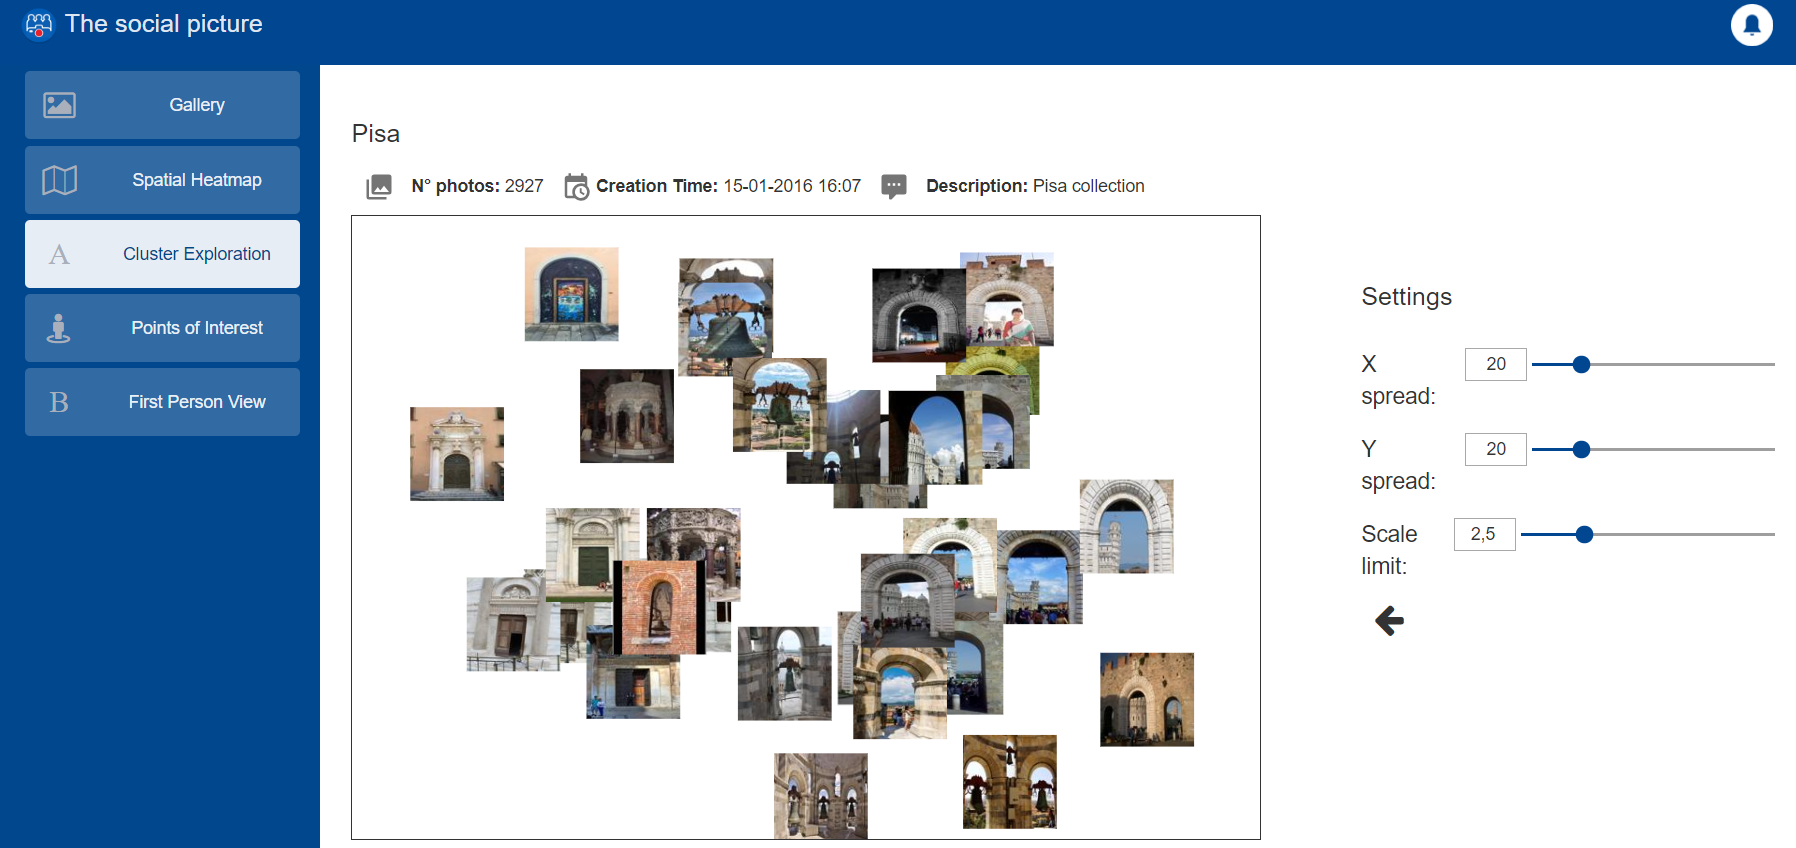
\includegraphics[width=1\linewidth]{archs.png}
	\caption{visualization interface for t-SNE based image embedding. In this example, a subset of images is shown. All the images are related to photos depicting \virgolette{archs}, however the group if images has been automatically created without taking into account the semantic of the images.}
	\label{tsneArchs}
\end{figure*}
As the number of pictures of a collection is unpredictable, the computation of the t-SNE coordinates could be very expensive. Besides the t-SNE computation, which needs to be executed only one time per dataset, a huge number of pictures can affect the browser efficiency for the visualization of the 2D embedding. We organize the entire collection of pictures in a hierarchical structure. After the collection is analysed (i.e., the \textit{fc7} features have been computed for all the images) the system performs a hierarchical k-means clustering of the image features. The algorithm divides the dataset recursively into \textit{k} clusters, for each computation the \textit{k} centroids are used as elements of a \textit{k-tree} and removed from the set. %Each node has \textit{k} children nodes (even empty), each one containing the cluster elements associated to the corresponding centroid. Since each node cannot contain more then \textit{k} elements, when this number is higher than \textit{k} the clustering is repeated recursively. 
When this new version of the t-SNE tool (hierarchical t-SNE) is executed, it shows to the user the t-SNE embedding computed only for the elements in the root of the \textit{k-tree} (i.e., the picture centroids of the first \textit{k-means} computation). When the user selects one of these pictures, the system computes the t-SNE of the pictures included in the child node corresponding to the selected picture element. This hierarchical exploration can be continued by selecting one of the shown pictures and computing the t-SNE embedding for its sub-elements in the hierarchy.
Figure~\ref{tsneArchs} shows an example of t-SNE visualization related to the group of images included in a child node of the tree. All these images are related to \virgolette{archs}, however it worth to highlight that this group has been automatically created without taking into account the semantic in the images, but only considering the pairwise distances between images of the entire collection and the implemented hierarchical organization.


\subsubsection{Other Advanced Tools}
%\begin{itemize}
%	\item Subsampling from set of images 
%	\item Captioning-Image Description:
%	with the aim to obtain better image descriptions, the system can generate a set of captions associated to each image. The dense captioning task generalizes object detection when the descriptions consist of a single word, and Image Captioning when one predicted region covers the full image \cite{Johnson2015densecap}. The result of dense captioning can be exploited to provide a description based image retrieval system, and an image description with an higher level of abstracton compared to the one given by an image classification approach.
%	\item Questions and Answers for assistive:
%	in the last few years, with the improvements in both natural language and image understanding, much effort has been spent by scientific community to develop algorithms for question answering on real-world images \cite{VQA}. These systems take and image and a natural language question about the image content, and provide a natural language answer. Such a system can be easily integrated in the \textit{The Social Picture} platform with the aim to improve its interfaces, allowing the visually impaired to know about the image collection's visual contents. The user is allowed to ask natural language questions about single images, the entire collections or an its subset.
%\end{itemize}
%
Among the tools included in \textit{The Social Picture} there is the one useful to generate automatic subsets of images from a specific photo collection. This tool allows the user to set the number of images to obtain as output for a collection in TSP, and automatically generates the subset of images taking into account visual features as well as EXIF information related to the images composing the photo collection (e.g., GPS location, TAGS, day, time, etc). In this way, the user can have some representative image prototypes related to the collection to be used for different purposes (e.g., printing the most significative pictures of paintings of a museum for a specific social group).

For each photo analysed by \textit{The Social Picture}, the system exploits three CNNs to extract information about object and places depicted, as well as determine if there is food in the picture (i.e., food vs. no-food classifier). Moreover, the automatic image captioning as described in~\cite{johnson2015densecap} is also exploited to extract a textual description from images. %With the aim to help the user to include a description to an uploaded image, \textit{The Social Picture} automatically generates and suggests a description to the user that can then refine it.  
The descriptions of images can be used for text based query performed by the user.
\begin{figure*}
	\centering
	%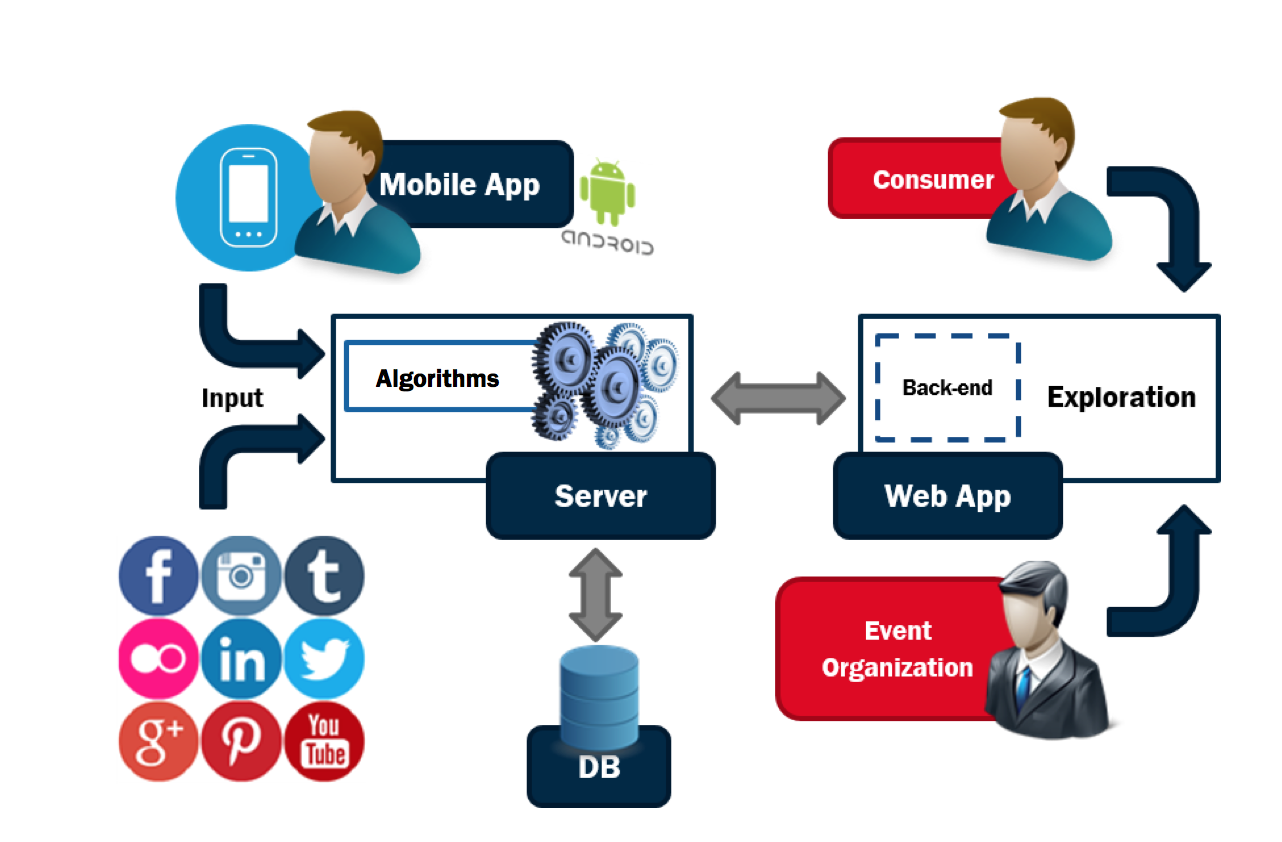
\epsfig{file=architecture.eps, width=2.72in}
	%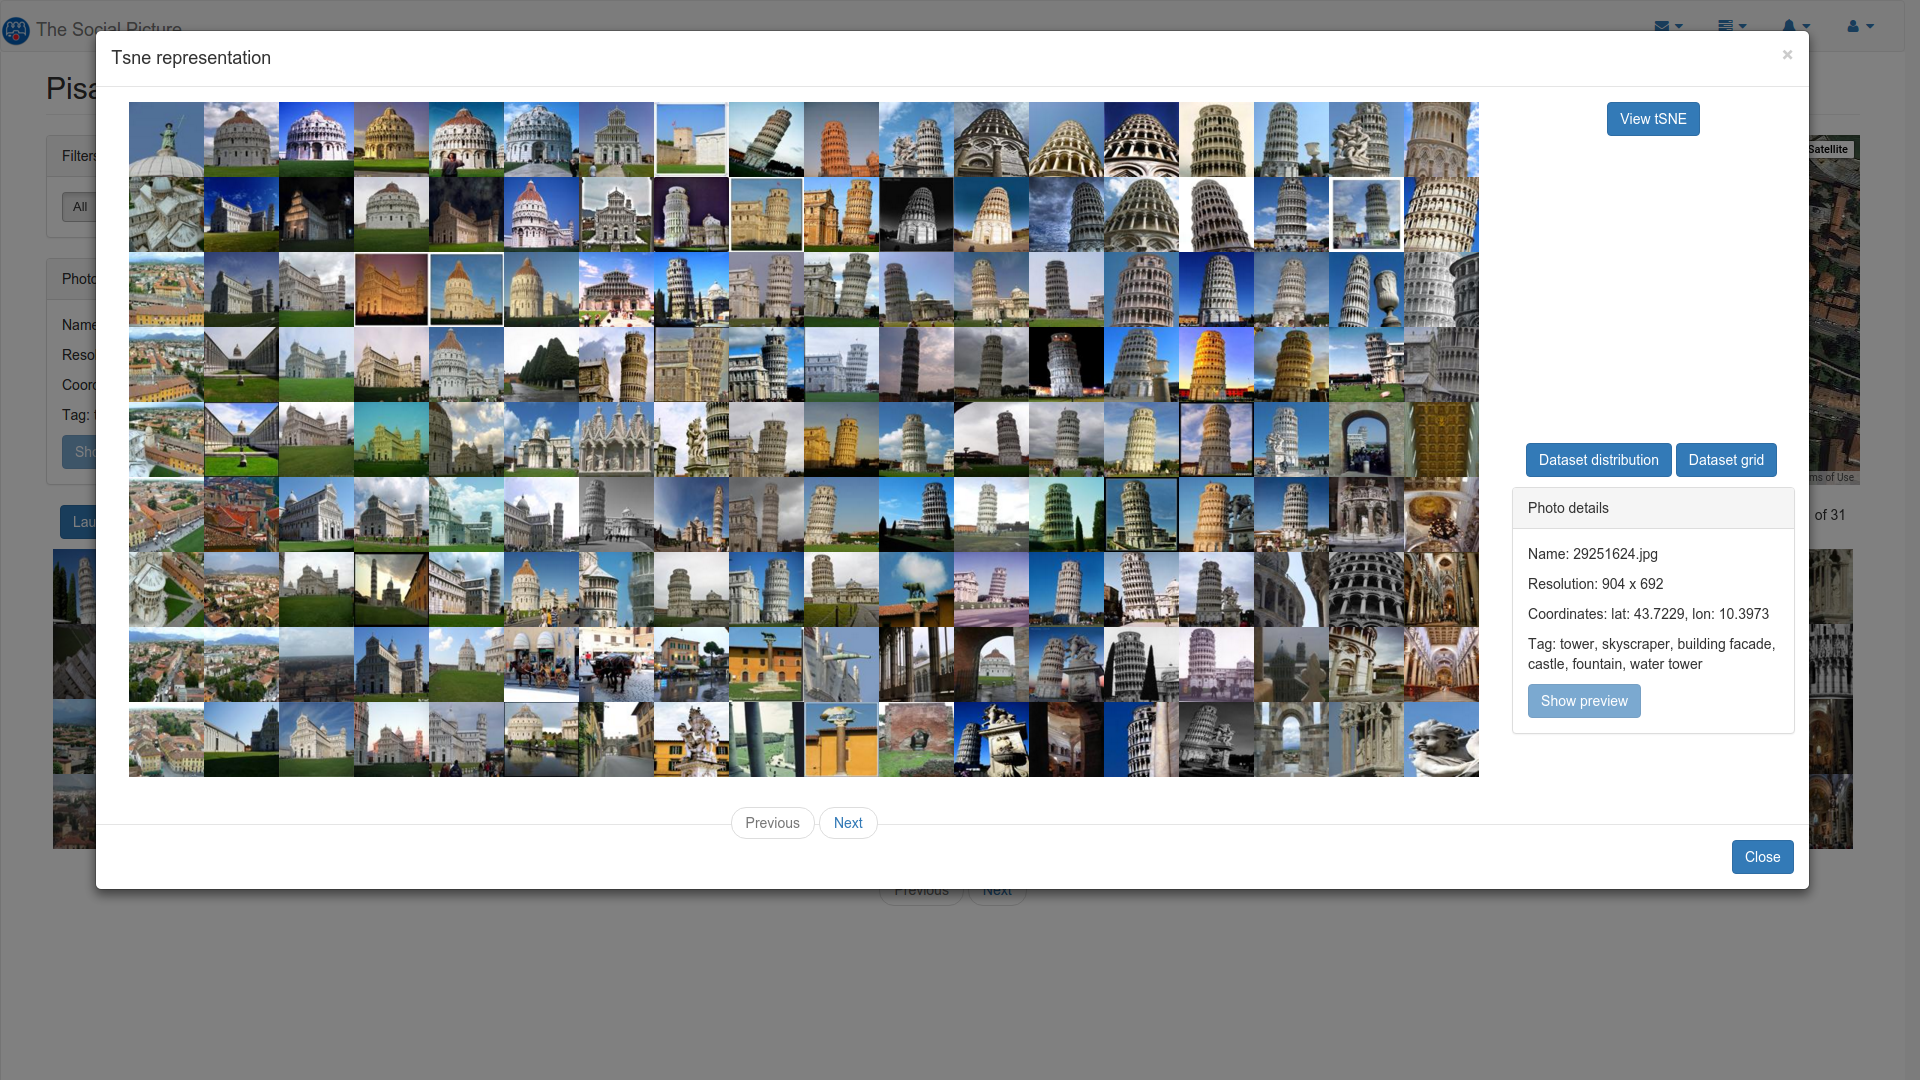
\includegraphics[width=1\linewidth]{gridtsne}
	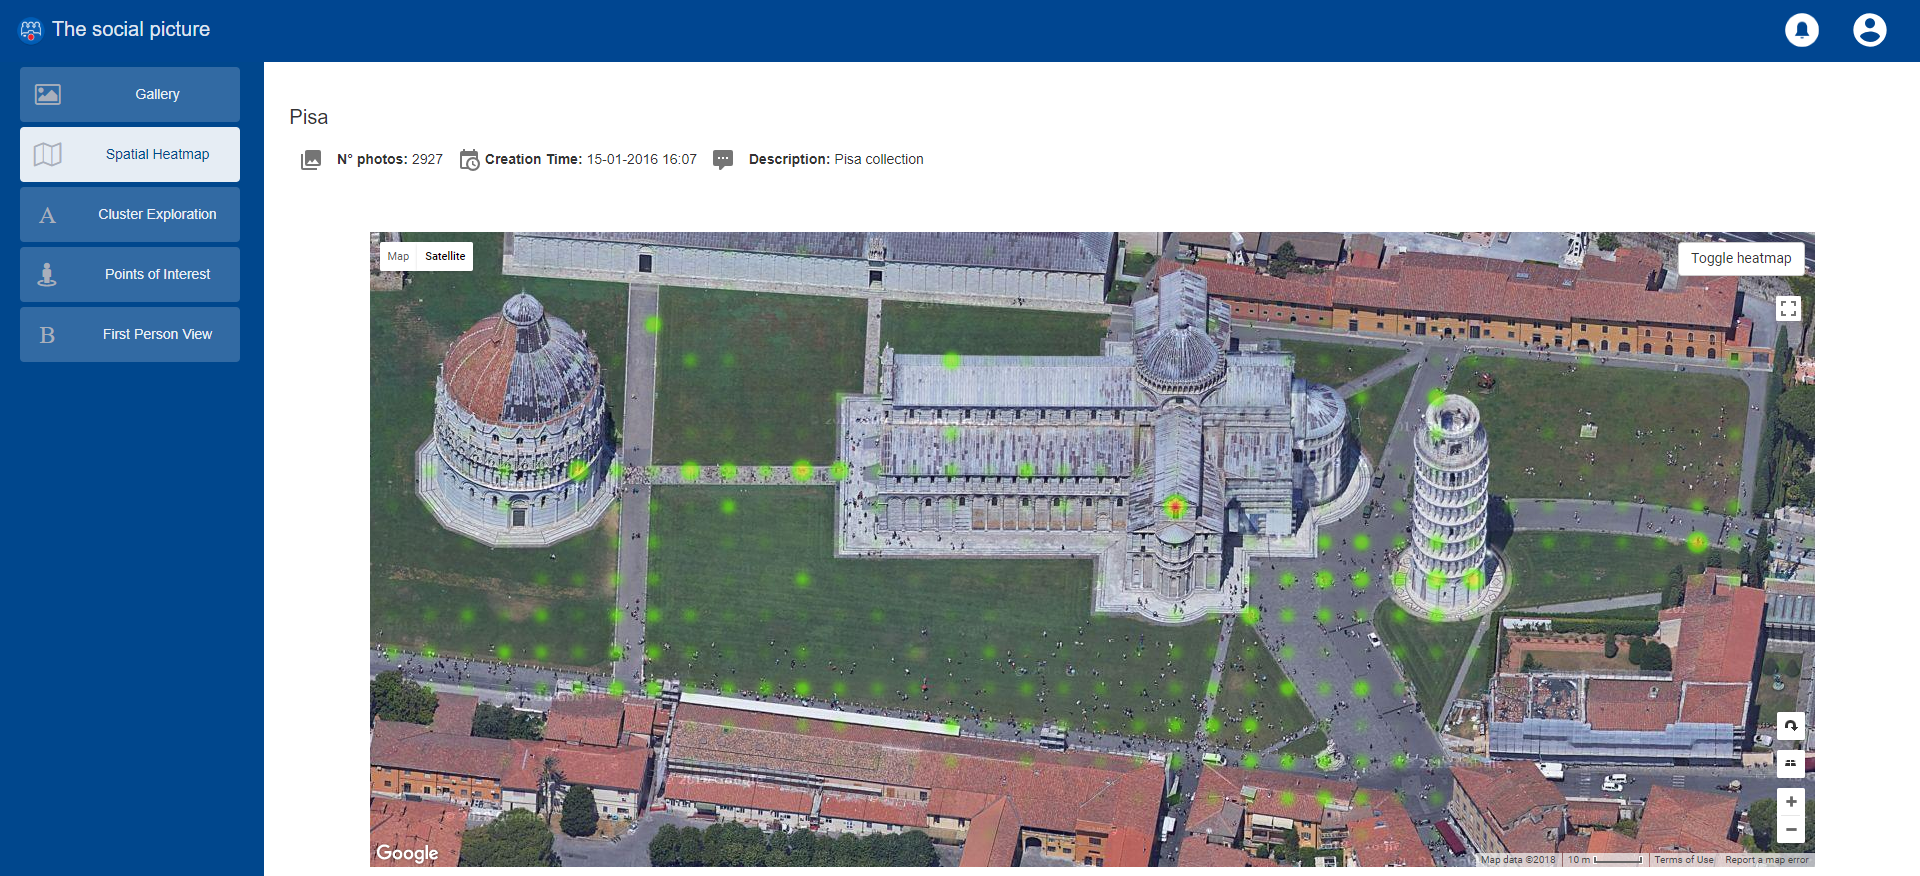
\includegraphics[width=1\linewidth]{map.png}
	\caption{visualization of the locations from which users taken the photos of the collection. This tool allow to understand how people visit the site and what are the places with the most popular point of views. By providing the positions of the users during the event it gives some hints about the most interesting parts of the site. }
	\label{mapGPS}
\end{figure*}

\subsection{Conclusions}
In this Chapter we discussed the Crowdsourced Media Analysis paradigm, as well as presenting a framework aimed to infer the interest of people attending an event or visiting a cultural heritage site based on the analysis of the taken photos.
Feedback about what is the most interesting part (i.e., the most captured) of a landmark building can help on taking decisions about renovating some parts rather than others as first investment.
The t-SNE exploration tool exploits a technique for feature space dimensionality reduction that is particularly well suited for the visualization of high dimensional image datasets. This tool allows the visualization of huge amount of pictures, and the hierarchical implementation allows to scale the number of analysed pictures. Very large collections can be explored, and the pictures are automatically arranged in semantic groups.
The system provides different exploration tools (e.g., heatmap, t-SNE exploration), automatic tagging engines (i.e., object classification, places, food vs. no-food, concept tags) and statistics. The extracted information can be exploited to define custom filters for images and to automatically infer how users act when visiting a cultural heritage site or attending to a public event, and what captured their interest. 


\chapter{Image Sentiment Analysis}\label{ch3}
\section{Introduction}
TSP --> POPOLARITA IMMAGINI SU BASE EVENTI/LUOGHI --> IMMAGINI RAPPRESENTATIVE
\\POLARITY --> SENTIMENT EVOCATO
\\POPULARITY --> POPOLARITA' SU PIATTAFORMA SOCIAL I.E. QUANTE PERSONE RAGGIUNGE\\
As instance, companies are interested in monitoring people opinions toward their products or services, as well as customers rely on feedbacks of other users to evaluate a product before they purchase it.
%For example, companies always want to find public or consumer opinions toward their products and services. Furthermore, customers also want to know the opinions of other users before they use a service or purchase a product.
With the growth of social media (i.e., reviews, forums, blogs and social networks), individuals and organizations are increasingly using public opinions  for their decision making~\cite{liu2012survey}.
%The analysis of such social information enables applications such as brand monitoring, market prediction or political voting forecasting.


The basic task in Sentiment Analysis is the polarity classification of an input text (e.g., taken from a review, a comment or a social post) in terms of positive, negative or neutral polarity. This analysis can be performed at document, sentence or feature level. The methods of this area are useful to capture public opinion about products, services, marketing, political preferences and social events. For example the analysis of the activity of Twitter's users can help to predict the popularity of parties or coalitions. The achieved results in Sentiment Analysis within micro-blogging have shown that Twitter posts reasonably reflect the political landscape~\cite{tumasjan2010predicting}.
Historically, Sentiment Analysis techniques have been developed for the analysis of text~\cite{pang2008opinion}, whereas limited efforts have been employed to extract (i.e., infer) sentiments from visual contents~(e.g., images and videos). % which are becoming a pervasive media on the web.
%Historically, the computational analysis of sentiment mostly concentrates on the textual contents~\cite{pang2008opinion}, whereas limited efforts have been conducted to analyse sentiments from visual contents such as images and videos, which are becoming a pervasive media type on the web.

Even though the scientific research has already achieved notable results in the field of textual Sentiment Analysis in different contexts (e.g., social network posts analysis, product reviews, political preferences, etc.), the task to understand the mood from a text has several difficulties given by the inherent ambiguity of the various languages (e.g., ironic sentences), cultural factors, linguistic nuances and the difficulty of generalize any text analysis solution to different language vocabularies. The different solutions in the field of text Sentiment Analysis have not yet achieved a level of reliability good enough to be implemented without enclosing the related context. For example, despite the existence of natural language processing tools for the English language, the same tools cannot be used directly to analyse text written in other languages.
In this Chapter we present three main inference tasks related to the image sentiment analysis that have been investigated in this research work: crowds behaviour, sentiment polarity, sentiment popularity. 

First, we present \textit{The Social Picture}~\cite{battiato2016social}, a framework to collect and explore huge amount of crowdsourced social images about public events, cultural heritage sites and other customized private events, with the aim to extract insights about the behaviour of people attending the same event or visiting the same place. 
Through \textit{The Social Picture} users contributes to the creation of image collections about common interests. %Users can add an image to a collection by using either a mobile application and a website interface. Furthermore, an event collection can be populated by selecting images from the most common social networks for images (e.g., Flickr, Panoramio, Instagram).
The collections can be explored through a number of advanced Computer Vision and Machine Learning algorithms, able to capture the visual content of images in order to organize them in a semantic way. The interfaces of \textit{The Social Picture} allow the users to create customized collections by exploiting semantic filters based on visual features, social network tags, geolocation, and other information related to the images.
Although the number of images could be huge, the system provides tools for the summary of the useful collection insights and statistics. It is able to automatically organize the pictures in semantic groups, according to several and live customizable criteria.
\textit{The Social Picture} can be used as a tool for analysing the multimedia activity of the audience of an organized event, or the activity of people visiting a cultural heritage site, performing inferences on the attitude of the participating people. The obtained information can be then exploited by the event organizers for the event evaluation and further planning or marketing strategies.

Then we present our work on the classic task of sentiment polarity prediction. Given an image, the proposed method properly combines visual and textual features to define an embedding space, then a classifier is trained on the embedded features. The novelty of the proposed method consists on the fact that we don't lean on the text provided by users, which is often noisy. Indeed we propose an alternative subjective source of text, directly extracted from images.
ABSTRACT

The third work presented in this Chapter is related to the task of image popularity prediction.
ABSTRACT

\section{The Social Picture}
\subsection{Introduction}
Images and videos have become one of the most popular media by which users express their emotions and share their experiences in the social networks. Nowadays the diffusion of social networks plays a crucial role in collecting information about people opinion and trends.
The proliferation of mobile devices and the diffusion of social media have changed the communication paradigm of people that share multimedia data by allowing new interaction models (e.g., social networks). In social events (e.g., concerts), the audience typically produces and share a lot of multimedia data with mobile devices (e.g., images, videos, geolocation, tags, etc.) related to what has captured their interest. The redundancy in these data can be exploited to infer social information about the attitude of the attending people. For example, systems such as RECfusion \cite{Ortis2015n525} can be developed to understand if there are groups of people interested to specific scenes. In the context of big social data, Machine Learning and Computer Vision algorithms can be used to develop new advanced analysis systems to automatically infer knowledge from large scale visual data \cite{weyand2015visual}, and other multimedia information gathered by multiple sources.

In this paper we introduce a framework called \textit{The Social Picture} (TSP) to collect, analyze and organize huge flows of visual data, and to allow users the navigation of image collections generated by the community.
We designed the system to be applied on three main scenarios: public events, cultural heritage sites, private events. TSP is a social framework populated by images uploaded by users or collected from other social media. The social peculiarities of such collections can be exploited not only by the people who partecipate to an event, in fact each scenario distinguishes two kind of users: the event organizer and the event partecipant.
Imagine an art-gallery manager who leases a famous Picasso's painting with the aim to include it in a event exhibition, together with other famous and expensive artworks. How does he know he did a good investment? Which was the more attractive artwork? From which position of the hall have people taken the most number of pictures?

These information can be inferred by analysing the multimedia audience activity (i.e., uploaded images) of the organized event in \textit{The Social Picture}. The collection of the uploaded images for an event, gives the sources analysed in TSP to answer the aforementioned questions. The obtained information can be then exploited by the event organizers for their event evaluation and further planning.

On the other hand, from the user point of view, the collection of an event can be exploited in a visualization tool which uses Computer Vision algorithms to organize images by visual content. In this way, the ``social picture'' of the event can be captured and shared among users.

In Figure \ref{heatmap}, an example of visual output produced by the proposed framework. It is computed by considering images automatically gathered from social media and related to the cultural heritage site of Teatro Massimo, in Catania. As detailed in the following sections, the interaction with the heat map allows the users to explore all the images contributing in each part of the analyzed cultural heritage site.
\begin{figure}
	\centering
	%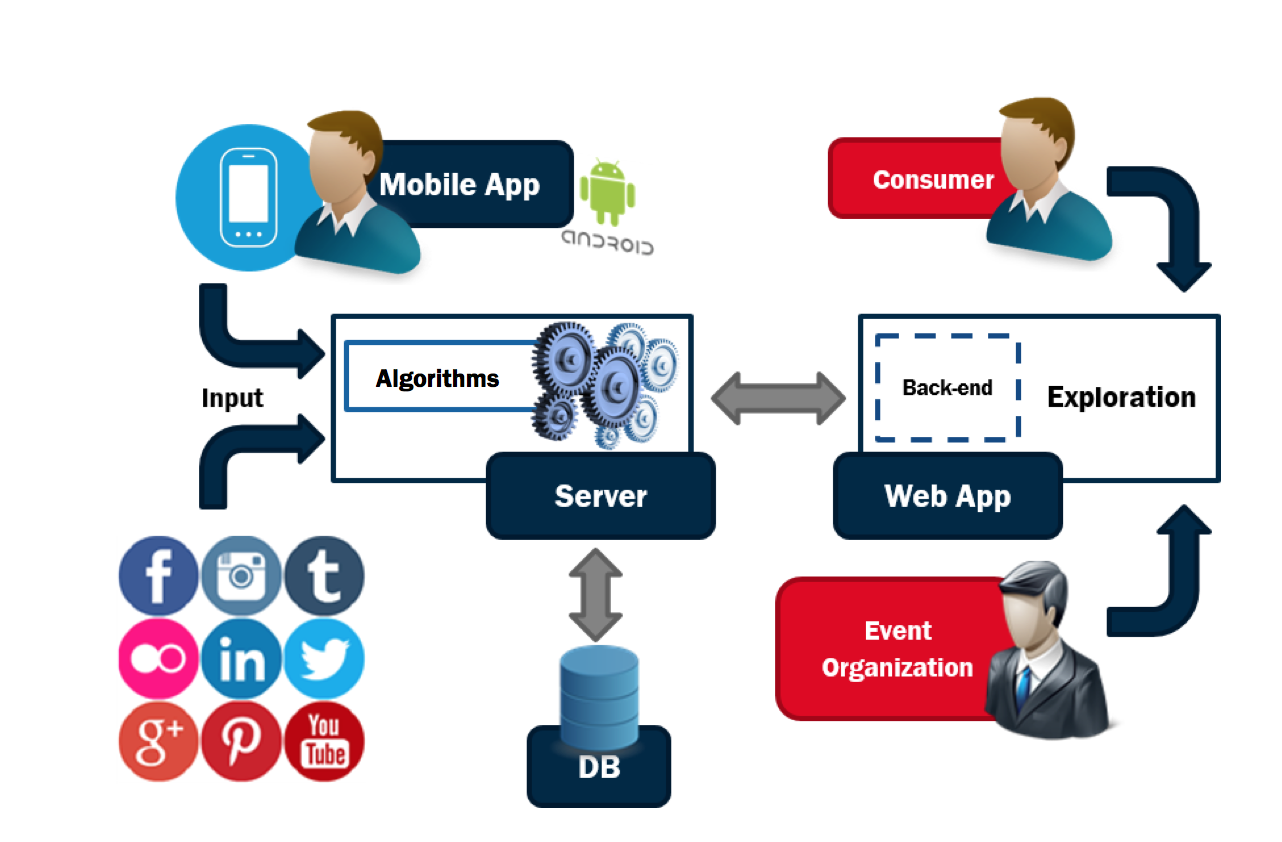
\epsfig{file=architecture.eps, width=2.72in}
	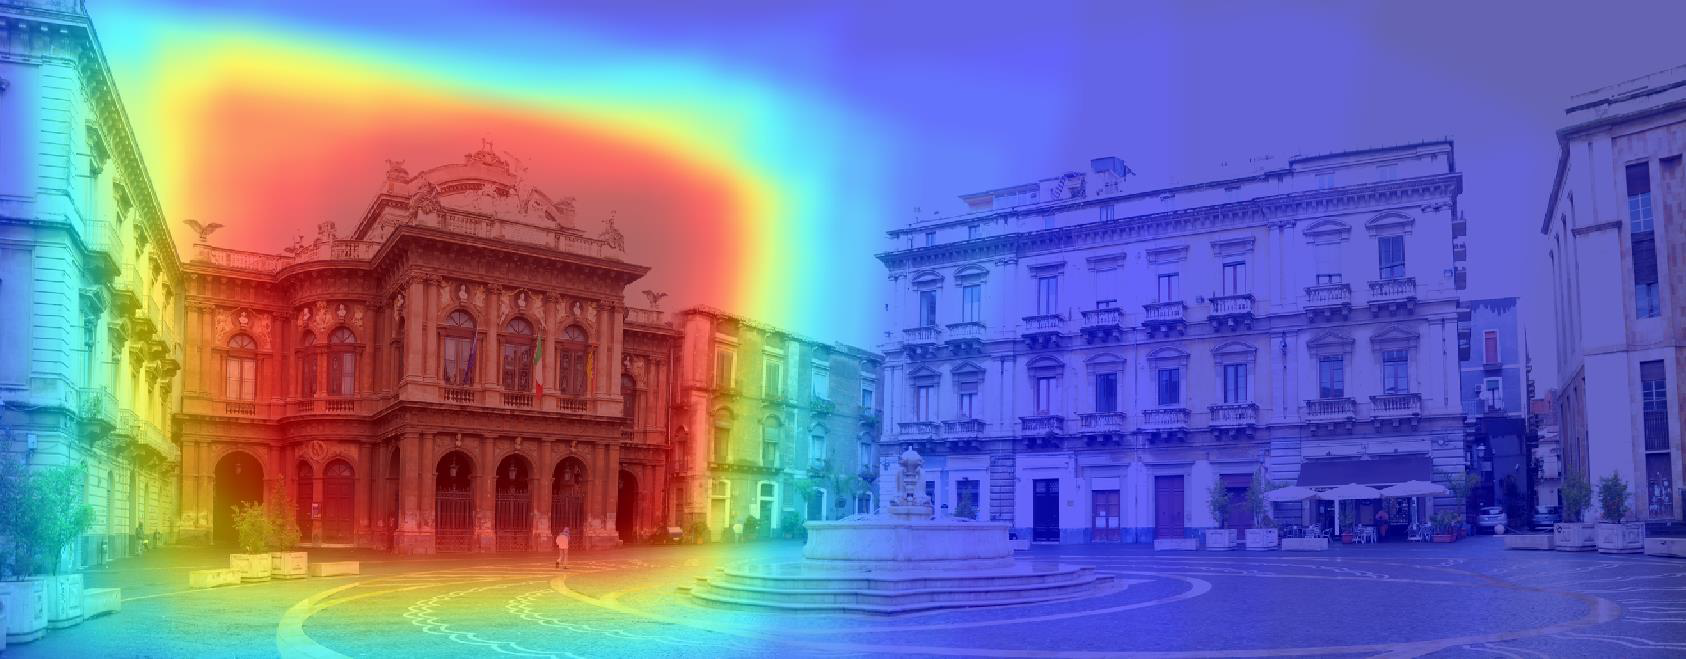
\includegraphics[width=1\linewidth]{heatmap}
	\caption{Heat map visualization.}
	\label{heatmap}
\end{figure}

\subsection{Architecture}
The architecture of the developed framework is shown in Figure \ref{architecture}.
Users can add an image to an event's collection by using a mobile application which gives access to \textit{The Social Picture} repository (TSP). The new images can be uploaded in TSP by using the mobile camera or by selecting images from the most common social networks for images (e.g. Flickr, Panoramio).
Once an image is uploaded, it is analysed by a set of Computer Vision algorithms, and then stored in the database together with the extracted features and the inferred high level attributes (e.g., type of scene recognized by the algorithm). These information are exploited in TSP to create smart interfaces for the users, which can be used during the exploration of the images related to an event's collection.
The framework collects all the data uploaded by the users of an event, and exploits this crowdsourced multimedia flow of pictures to infer social behavioural information about the event considering the popularity of the uploaded scenes \cite{Ortis2015n525}.

The collections can be explored from smartphones, tablet or desktop computers via a web application, which exhibits a range of filtering tools to better explore the huge amount of data (see Figure \ref{interface}).
%\subsubsection{Database}
%When a new image is added to the system, it is analysed by a set of algorithms with the aim to extract pre-defined features (both visual and textual), as well as semantic information. The image is collected, entered, processed and all the analysis results are stored in the Database. 
%\subsubsection{Mobile App}
%The mobile application allows users to upload their visual contributes to the event's collection. Other users can also contribute to the creation of the collection by posting their contents through the considered social netwoks, by adding a specific event's hashtag.
%\subsubsection{Web Application}
The web application shows different interfaces depending of the specific user and the event in which he has joined after an invitation from the event manager (the person who created the event). To join an event's collection, the user must upload at least one picture related to that event. Collections can be explored by several data visualization enviroments, which are selected by the event manager. Anyone registered to \textit{The Social Picture} can become event manager and start a social collection: this follows the ``prosumer'' paradigm, where the users are both producers and consumers of the service.
The developed framework is characterized by a modular architecture: new visualization interfaces, as well as new semantic filters can be independently created and futher added to the system. 
Thus, when an event manager creates a new collection, he is allowed to specify several options to customize the image gathering, the social analysis to be performed and the visualization tools for the users of that collection.
The event manager is also allowed to set a range of statistics, which will be available after the analysis of the collected images. These statistics helps organizators to extract useful social information from the crowdsourced pictures \cite{Milotta2016n544}. For example, what is the most popular artwork of a museum? What is the least considered? From which perspective these pictures were taken?
These information could be exploited, for example, to perform aimed investments. The system can suggest what is the better subject to use for the advertising campaign of the event, or which of the attractions it worth to mainly reproduce in the souvenir shop products, to support merchandising strategies. Feedback about what is the most interesting part (i.e., the most photo captured) of a landmark building can help on taking decisions about renovating some parts of the building rather than other as first investment, where the connotation of importance is achieved by the crowd who generated ``the social picture'' for that building by uploading related images.
\begin{figure}
%	\vspace{-0.3in}
	\centering
	%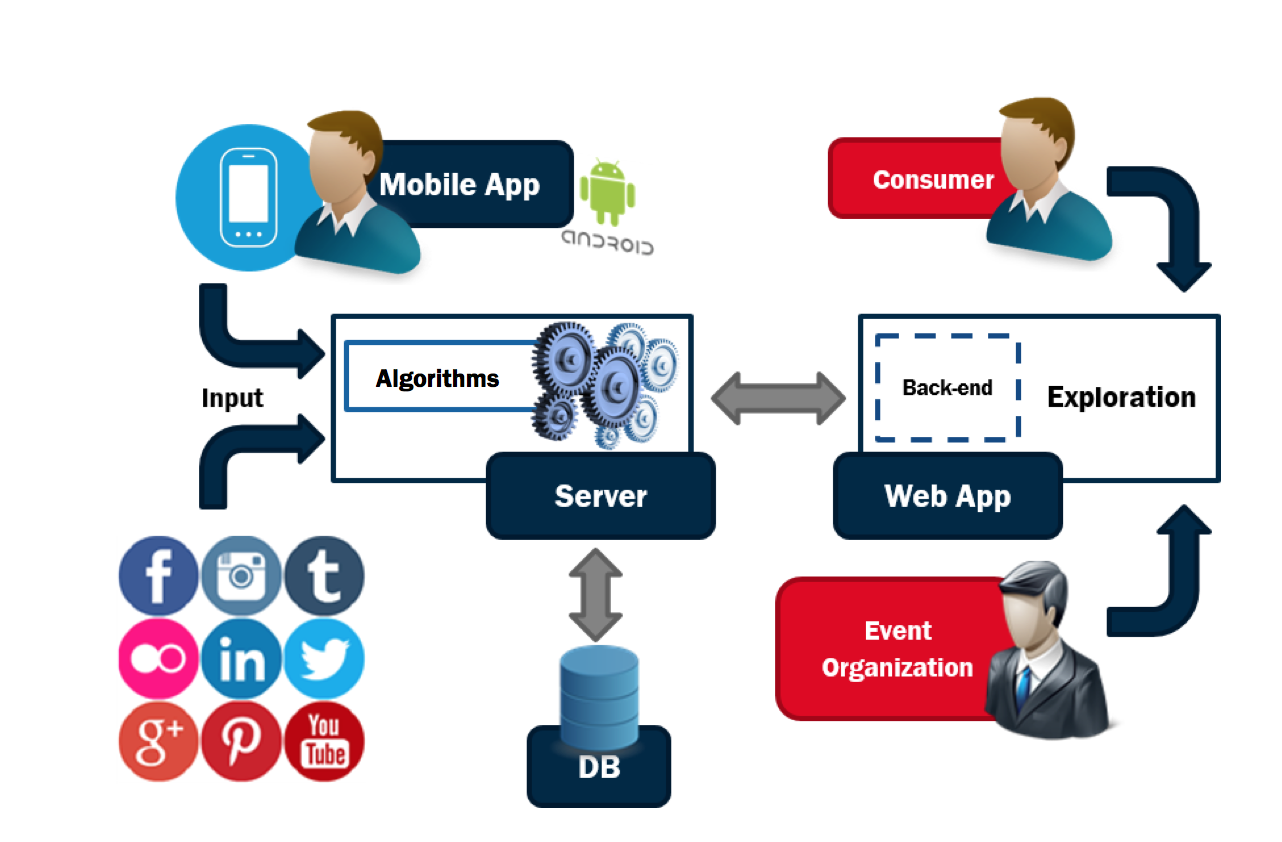
\epsfig{file=architecture.eps, width=2.72in}
	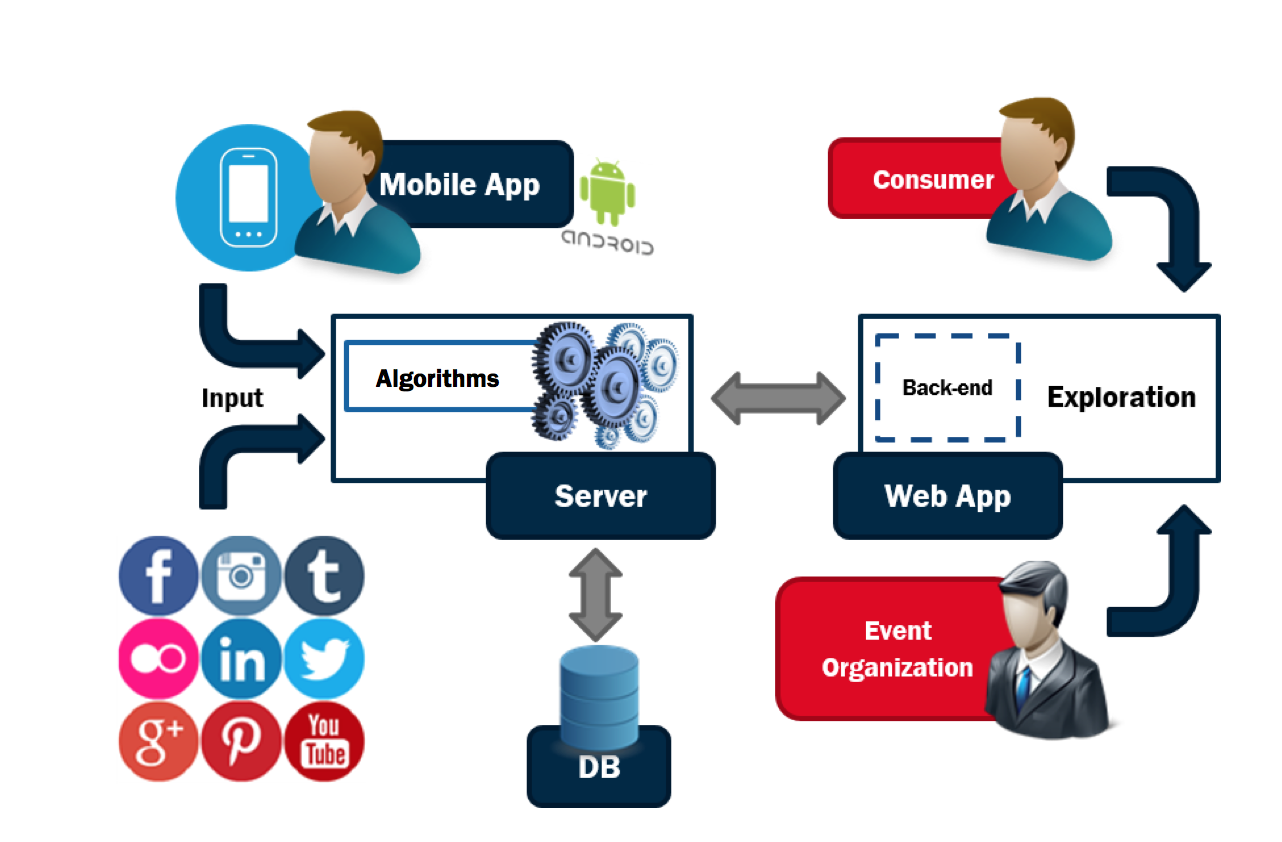
\includegraphics[width=0.7\linewidth]{architecture}
	\caption{The Social Picture's architecture.}
	\label{architecture}
\end{figure}

\begin{figure*}
	\centering
	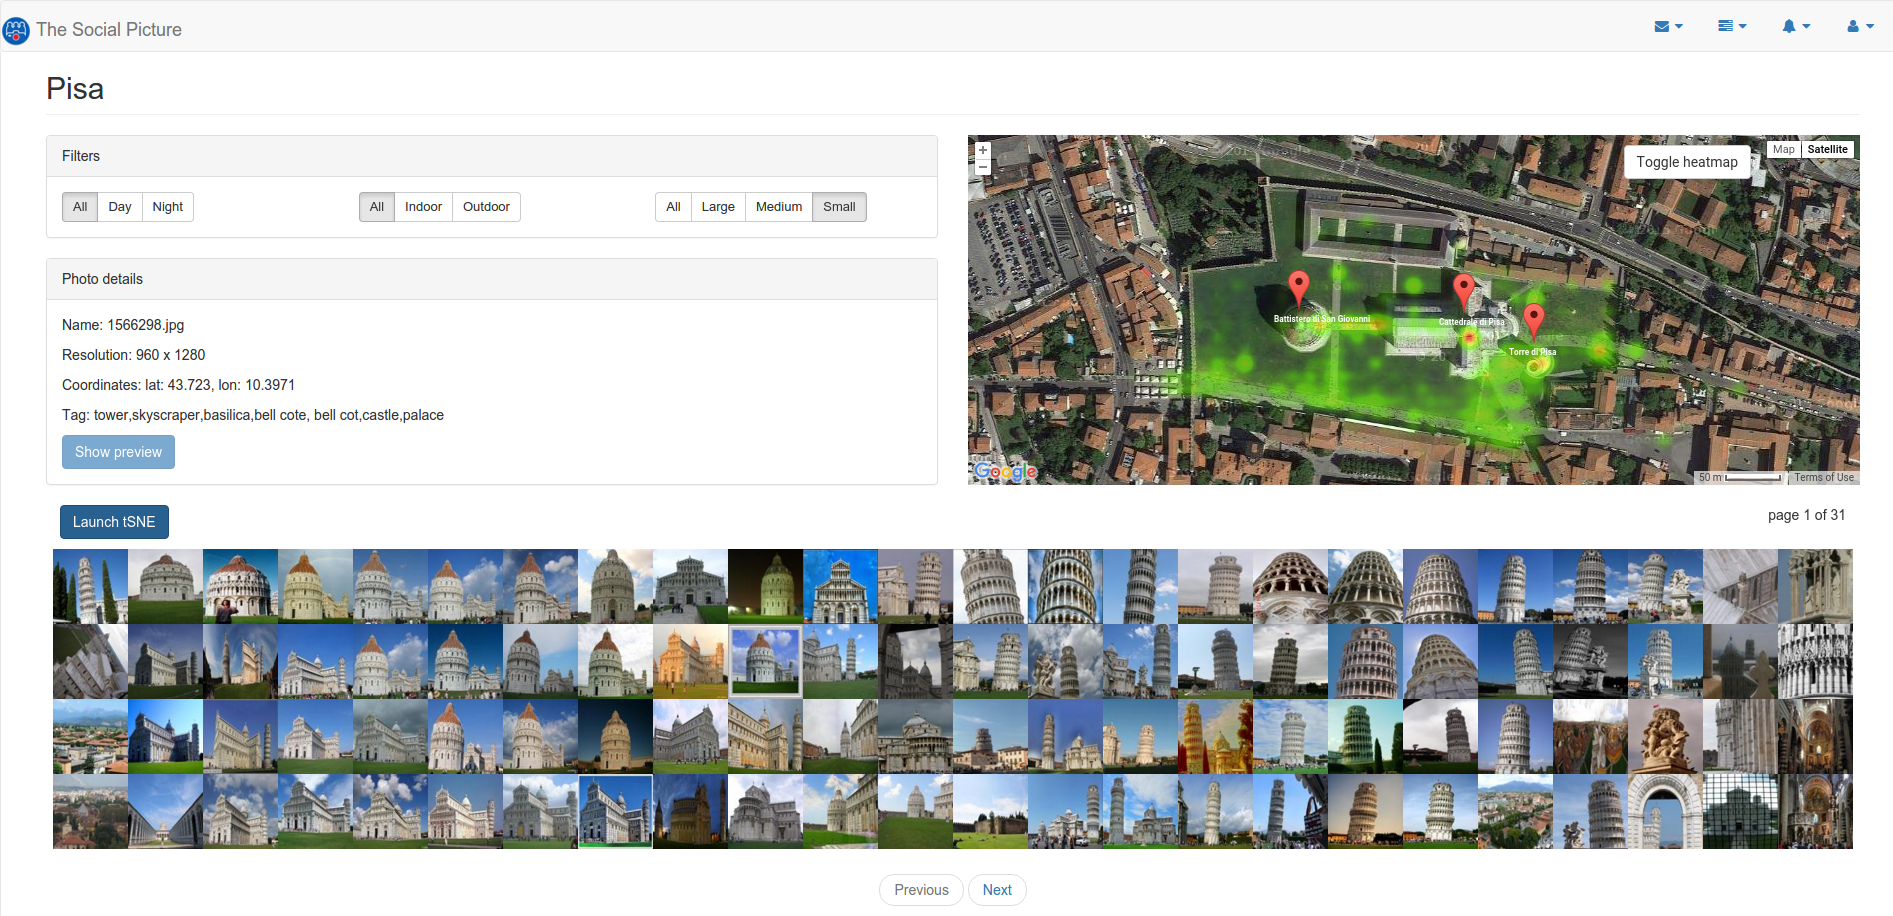
\includegraphics[width=1\linewidth]{interface01}
	\caption{Example of exploration interface. It is composed by three main areas: the map area (upper-right) shows the positions where the images have been taken from. This give the positions of the users during the event and some hints about the most interesting parts of the site. The interaction with this map allows the users to know more details by selecting the images from their positions. The gallery (bottom) shows the collection's pictures organized by using t-SNE algorithm according to the selected filters and allows the users to explore the collection. The detail area (upper-left) shows the details of a picture selected from the gallery, and presents the available filters.
		From this interface, the user can launch the t-SNE algorithm on a customized set of images, apply one or more filters, and know more about the different statistics and inferences performed by the system.}
	\label{interface}
\end{figure*}

%\subsubsection{Analysis engine}
The several exploration tools are based on both visual and textual data. The system exploits information such as Exif data (camera model, geolocalization, acquisition details, JPEG compression, and others) when available, and a number of ad hoc extracted visual features.

The visual analysis module of the system feds all the images to two different CNNs \cite{krizhevsky2012imagenet, zhou2014learning}, in order to extract the classification labels and an image representation. To attach semantic labels to the visual content of the images, we used \textit{AlexNet} \cite{krizhevsky2012imagenet} and \textit{Places205-AlexNet} \cite{zhou2014learning}.
The CNN used in \cite{krizhevsky2012imagenet} consist of seven internal layers with a final 1000-way softmax which produces a distribution over the 1000 predefined classes of the ImageNet dataset \cite{ILSVRC15}.We considered the feature activations induced at the last hidden layer, which consists of 4096 dimensional feature (fc-7 feature), as an image representation to be further used with t-SNE algorithm \cite{van2008visualizing} for visualization purposes. 
We also fed the images to the \textit{Places205-AlexNet} CNN \cite{zhou2014learning}. This CNN has the same architecture of \textit{AlexNet} CNN, but it is trained on 205 scene categories related to places learned by using the database \textit{Places205-AlexNet} composed by 2.5 million images.

%The results of the image evaluation by the above CNNs consist of the three classification predictions with the highest scores, given by each CNN, and the fc7 image representation.
\subsection{User experience}
An event manager (i.e., a user of \textit{The Social Picture} which starts a new collection) creates a new event by selecting among three possible type of event: public event (e.g., a concert), cultural heritage site (e.g., a museum) or private event (e.g., a wedding). The available event categorization can be extended to include other customized categories. We considered these three categories to better focus the aims of the specific analysis, and the inferred information that an organizator wants to extract.
The data gathering from users can be performed within a specific time window. The manager is allowed to control the image acquisition by selecting fine-grained criteria such as filtering media by hashtag, associated text or geolocalization distance.
After creating the event and its acquisition settings, the manager can select the statistics that the system have to compute by exploiting the collection of multimedia data gathered for that event.

The pictures can be grouped by hierarchical categories depending on the combination of two or more of the extracted visual features, which allow us to create several taxonomies in the image collection (panoramic pictures versus close-ups, natural versus artificial, indoor or outdoor, the presence or absence of crowds, selfies versus not selfies, and others).
Specific image categorizations help users to better handle huge amount of crowdsourced pictures, this kind of grouping can be exploited as a pre-processing before performing an image based visual search. Given a seed image, the system selects a set of similar pictures.
The system provides different exploration tools. There is a tool for the exploration of outdoor collections such as cultural sites. % and whenever a large environment image can be considered as a reference for more detailed ones,
One more tool can be exploited to better navigate any huge image collection. These exploration tools together with other advanced tools are described in the next subsections.
A video of the demo is available at the following link:
http://iplab.dmi.unict.it/TSP

\subsubsection{Heat map exploration}
In a cultural heritage site, people usually take pictures from different points of view and considering different details of parts related to famous and appreciated attractions and artworks. The heat map exploration tool of \textit{The Social Picture} aims to infer the ``interest'' of people with respect to the different parts of a site. An example of heat map generated from data in \textit{The Social Picture} is shown in Figure \ref{heatmap}. Through this visualization tool, an organizer of a collection will be able to know which parts of the site captures people's interests.
On the other hand, users can explore the collection related to a site in a very simple and intuitive way. So, to highlight the ``interest'' of people related to parts of a site, the proposed system creates an heat map by aligning images in \textit{The Social Picture} with respect to panoramic images of the site of interest~\cite{Mikulik2015}.

The heat map is a visualization used to depict the intensity of images at spatial points. The heat map consists of a colored overlay applied to the original image. Areas of higher intensity will be colored red, and areas of lower intensity will appear blue. The intensity of the heat map is given by the number of collected pictures that contain that visual area.
By clicking on a point of the heat map, the user can visualize the subject of images that contribuited to generate the map intensity at that point. This set of pictures can be further refined by selecting one of the images and asking the system to search similar pictures, or use the image subset as a starting point for furhter analysis. In other words, the heat map visualization gives the possibility to understand the behaviour of the people. Also it can be considered as a powerful and intuitive image retrieval tool for the collections related to cultural heritage sites.

\begin{figure*}
	\centering
	%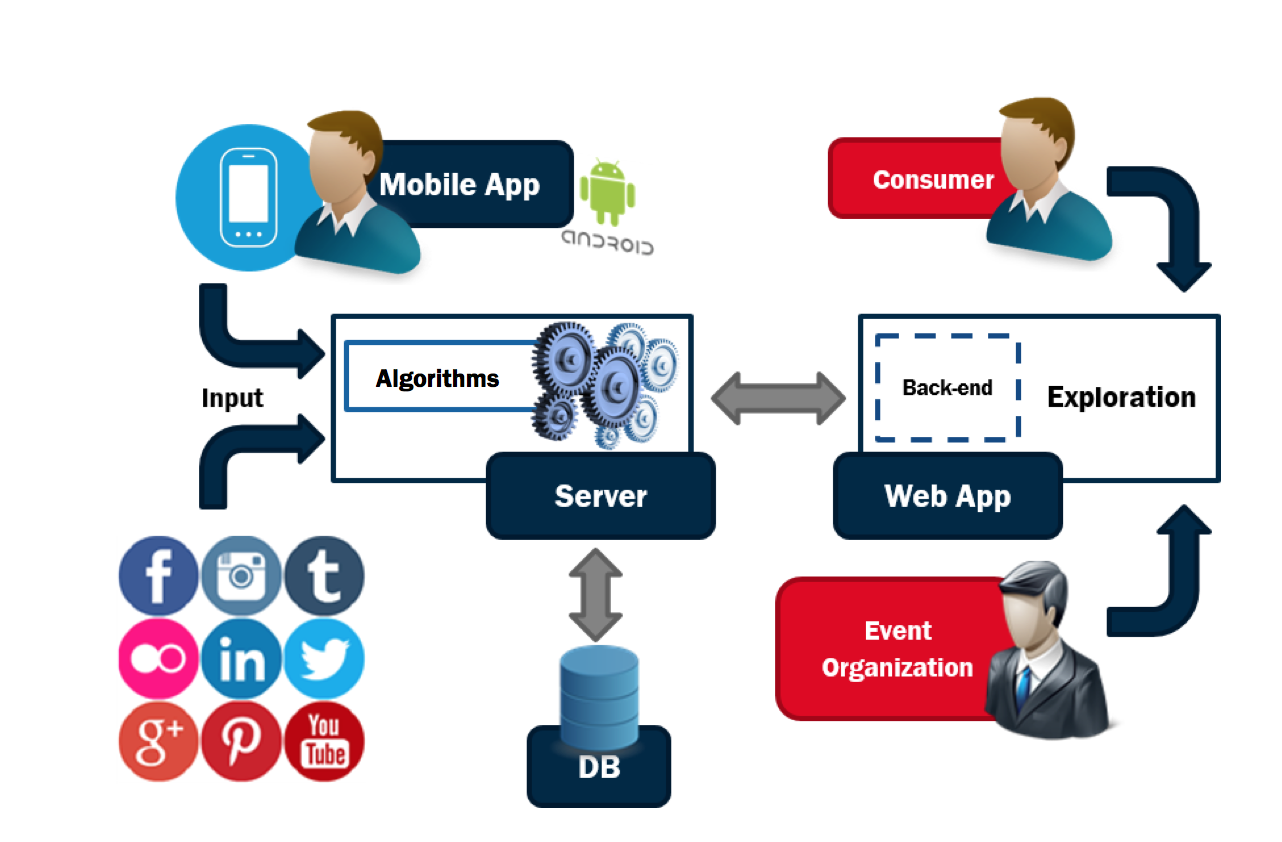
\epsfig{file=architecture.eps, width=2.72in}
	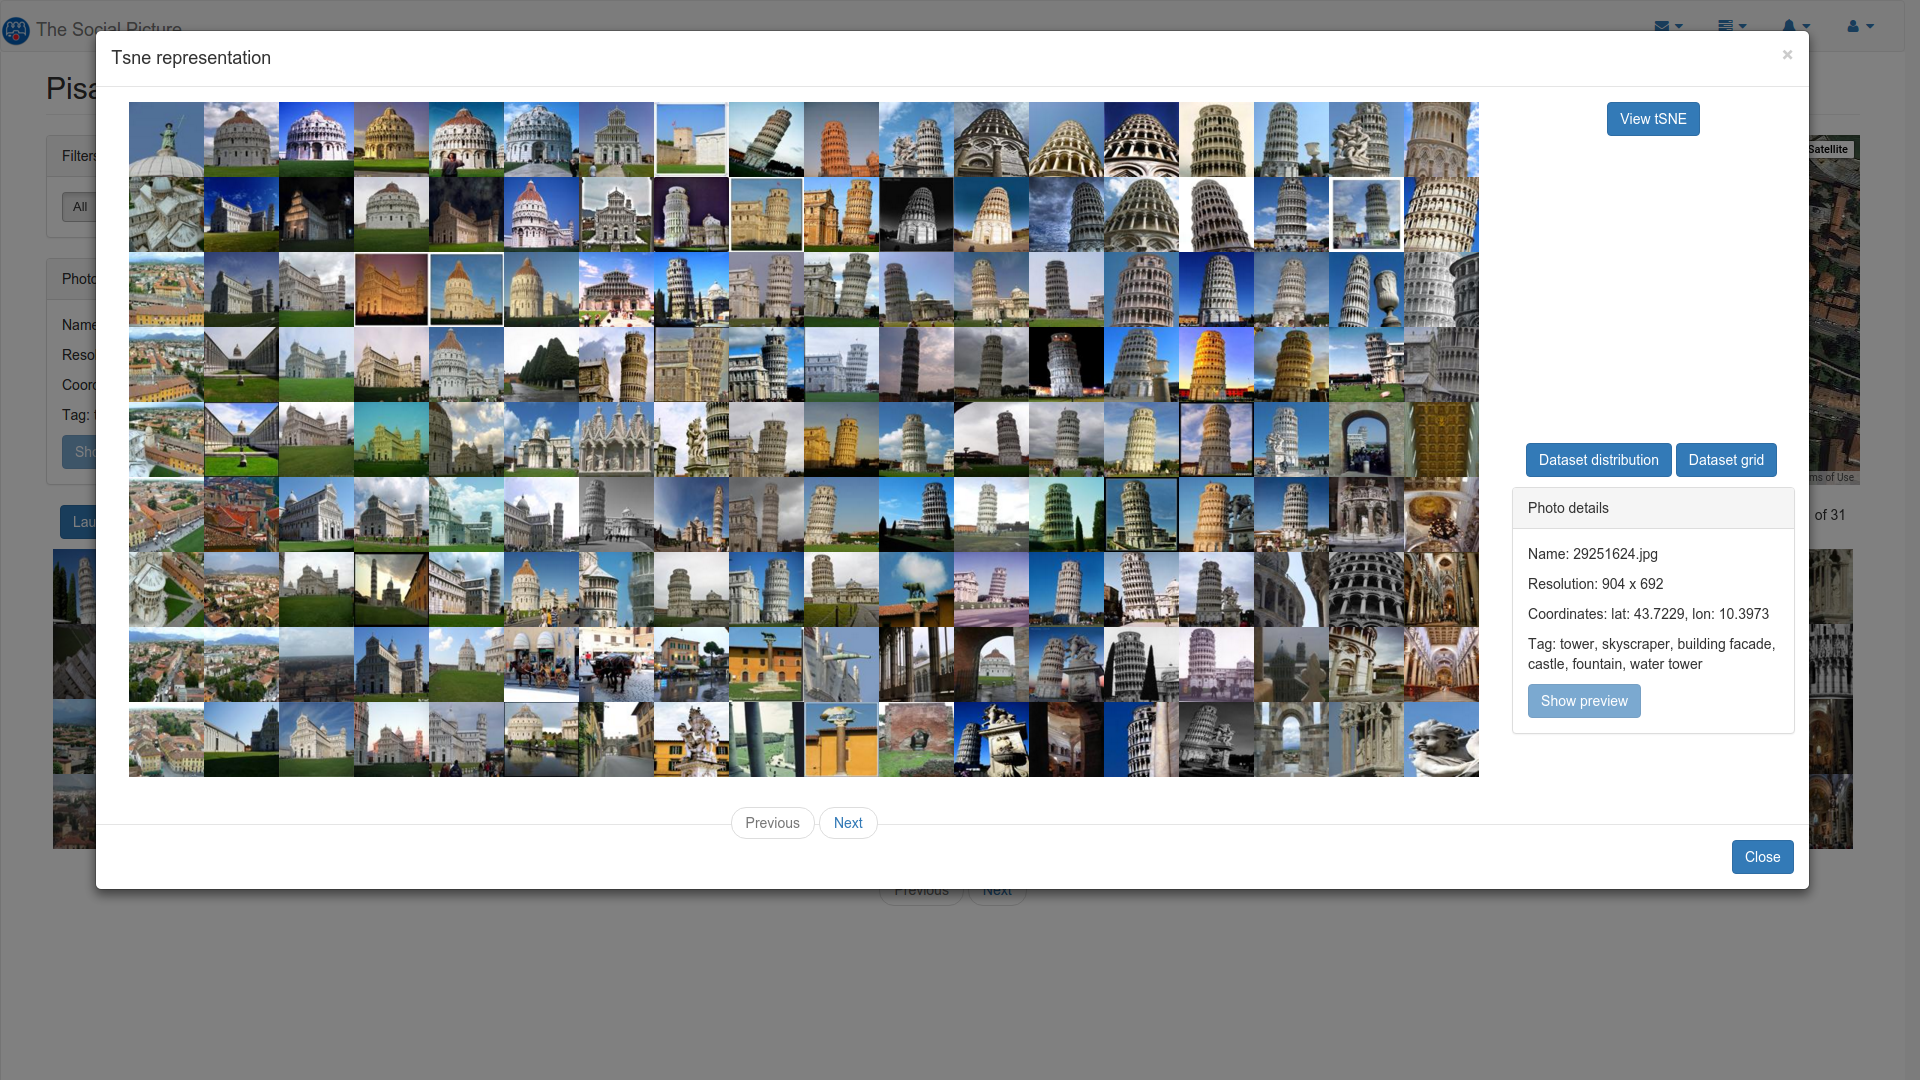
\includegraphics[width=1\linewidth]{gridtsne}
	\caption{t-SNE visualization, the images are forced to fit a grid layout. Images of an event are automatically organized by visual content. Images close in the 2D space of the visualization tool are also close in terms of visual content.}
	\label{gridtsne}
\end{figure*}

\paragraph{3D Reconstruction}
Starting from VSFM (Visual Structure From Motion)~\cite{wu2013towards}, we are able to compute a 3D sparse reconstruction of large photos collections. The models are augmented with colors for vertices, related to the frequency of been acquired in a photo, colors for cameras, related to the number of visual features acquired by each photo, and with a plane which show the spatial density of contributing users. We embedded in TSP the models through a 3D web viewer based on Threejs, allowing the users to browse the 3D sparse reconstructed models gaining a cue about what are the points of view and the subjects preferred by users when take photos. Moreover, the models in the 3D web viewer can also be browsed through Leap Motion system, an intuitive and fast interactive system.
\vspace{-0.2cm}


\subsubsection{t-SNE exploration}
We exploit the fc7 feature extracted with the \textit{AlexNet} architecture \cite{krizhevsky2012imagenet} for each image and use the t-SNE embedding algorithm \cite{van2008visualizing} to compute a 2D embedding that respects the pairwise distances between visual features, forcing to fit a grid layout (Figure \ref{gridtsne}). The t-SNE (t-Distribuited Stochastic Neighbour Embedding) is a technique for feature space dimensionality reduction that is particularly well suited for the visualization of high dimensional image datasets.
Note that images with the same subject are automatically arranged nearby (see Figure \ref{gridtsne}). Moreover, the system arranges very close those images which are not the same but have a similar visual content. It is also important to highlight that the employed CNN \cite{krizhevsky2012imagenet} has been trained using a different dataset concerning 1000 classes of objects, but the fc7 features resulted expressive and representative enough to be applied succesfully to a generic event collection.

%Another exploration tool, allow users to see the result of t-SNE embedding without using the grid layout. If we display a set of images using their embedded locations computed by t-SNE, they may overlap one each other. Especially if there are many similar images. For this reason, this interface provides a set of tools to help the user's navigation.

With this exploration tool, the user can apply a translation or a zooming to all the viewed images, just clicking and dragging the mouse along the desidered direction and by using the scroll wheel respectively. This helps the user to better explore the image distribution in a custom level of detail.
%A number of tools enable users to fine-tune the spread of images along X and Y axis, and the zooming effect. These parameters can be used to transform the distribution of the embedded images, and adapt the effect of the mouse commands. For example, if the user fix an upper bound for the zoom effect, when this limit is reached the scrool wheel of the mouse has the effect of separating the images according to the amout of the rotation.
Furthermore, the user can choose a subset of images and compute the t-SNE embedding of them directly on the browser (see Figure \ref{gridtsne}).% This tool has been developed by using the \textit{tsnejs} Javascript library by Andrej Karpathy.

\paragraph{Hierarchical t-SNE}
The first implementation of the t-SNE exploration tool in TSP was unable to scale with the number of the collections' images. The new tool presented in this demo implements an hierarchical version of the t-SNE embedding which allows to explore picture collections without limits on the amount of processed pictures. 
This helps the user to better explore the image distribution in a custom level of detail. Furthermore, the user can choose a subset of images and compute the t-SNE embedding of them directly on the browser. % This tool has been developed by using the \textit{tsnejs} Javascript library by Andrej Karpathy.
As the number of pictures of a collection is unpredictable, the computation of the t-SNE coordinates could be very expensive. Besides the t-SNE computation, which needs to be executed only one time per dataset, a huge number of pictures can affect the browser efficiency for the visualization of the 2D embedding. We organize the entire collection of pictures in a hierarchical structure. After the collection is analysed (i.e., the \textit{fc7} features have been computed for all the images) the system performs a hierarchical k-means clustering of the image features. The algorithm divides the dataset recursively into \textit{k} clusters, for each computation the \textit{k} centroids are used as elements of a \textit{k-tree} and removed from the set. %Each node has \textit{k} children nodes (even empty), each one containing the cluster elements associated to the corresponding centroid. Since each node cannot contain more then \textit{k} elements, when this number is higher than \textit{k} the clustering is repeated recursively. 
When this new version of the t-SNE tool (hierarchical t-SNE) is executed, it shows to the user the t-SNE embedding computed only for the elements in the root of the \textit{k-tree} (i.e., the picture centroids of the first \textit{k-means} computation). When the user selects one of these pictures, the system computes the t-SNE of the pictures included in the child node corresponding to the selected picture element. This hierarchical exploration can be continued by selecting one of the shown pictures and computing the t-SNE embedding for its sub-elements in the hierarchy.



\subsubsection{Other Advanced Tools}
%\begin{itemize}
%	\item Subsampling from set of images 
%	\item Captioning-Image Description:
%	with the aim to obtain better image descriptions, the system can generate a set of captions associated to each image. The dense captioning task generalizes object detection when the descriptions consist of a single word, and Image Captioning when one predicted region covers the full image \cite{Johnson2015densecap}. The result of dense captioning can be exploited to provide a description based image retrieval system, and an image description with an higher level of abstracton compared to the one given by an image classification approach.
%	\item Questions and Answers for assistive:
%	in the last few years, with the improvements in both natural language and image understanding, much effort has been spent by scientific community to develop algorithms for question answering on real-world images \cite{VQA}. These systems take and image and a natural language question about the image content, and provide a natural language answer. Such a system can be easily integrated in the \textit{The Social Picture} platform with the aim to improve its interfaces, allowing the visually impaired to know about the image collection's visual contents. The user is allowed to ask natural language questions about single images, the entire collections or an its subset.
%\end{itemize}
%
Among the tools included in \textit{The Social Picture} there is the one useful to generate automatic subsets of images from a specific photo collection. This tool allows the user to set the number of images to obtain as output for a collection in TSP, and automatically generates the subset of images taking into account visual features as well as EXIF information related to the images composing the photo collection (e.g., GPS location, TAGS, day, time, etc). In this way, the user can have some representative image prototypes related to the collection to be used for different purposes (e.g., printing the most significative pictures of paintings of a museum for a specific social group).

One more feature included in The Social Picture is the automatic image captioning as described in~\cite{johnson2015densecap}. With the aim to help the user to include a description to an uploaded image, \textit{The Social Picture} automatically generates and suggests a description to the user that can then refine it.  The descriptions of images can be used for text based query performed by the user.


\section{Image Polarity Prediction}

\section{Image Popularity Prediction}

\section{Conclusions}
\chapter{Video Sentiment Analysis}

\section{Introduction}

\section{RECfusion}

\section{RECfusion for lifelogging}

\section{Conclusions}
\chapter{Final Discussion, Remarks and Future Works}\label{ch2}

%----------------------------------------------------------------------------------------
%	THESIS CONTENT - APPENDICES
%----------------------------------------------------------------------------------------
%
%\appendix % Cue to tell LaTeX that the following "chapters" are Appendices
%
%% Include the appendices of the thesis as separate files from the Appendices folder
%% Uncomment the lines as you write the Appendices
%
%\include{Appendices/AppendixA}
%%\include{Appendices/AppendixB}
%%\include{Appendices/AppendixC}

%----------------------------------------------------------------------------------------
%	BIBLIOGRAPHY
%----------------------------------------------------------------------------------------

%\bibliography{refs}
%\bibliographystyle{unsrt}
\printbibliography[heading=bibintoc]
%\printbibliography



%----------------------------------------------------------------------------------------

\end{document}  
